\documentclass{whutmod}
\usepackage{metalogo}
\usepackage{float}
\usepackage{subfigure} 
\usepackage{url}
\usepackage{booktabs}
\usepackage[style=caspervector,backend=biber,utf8]{biblatex}
\addbibresource{wenxian.bib}
\team{23}
\membera{刘子川}
\joba{编程}
\memberb{程宇}
\jobb{建模}
\memberc{陈荣兴}
\jobc{建模}
\hypersetup{
	colorlinks=true,
	linkcolor=black
}

\title{第四次论文格式}
\tihao{4} 

\begin{document}

%	\maketitle
	
	\begin{abstract}
“拍照赚钱”APP 是基于移动互联网的自助式劳务众包平台,使得企业可利 用大众力量,低成本、高效率地完成各种商品检查与信息搜集的任务。本文通过 建立数学模型,就 APP 中的任务定价问题进行分析,给出最优的任务定价方案。
   ~\\%~\\为换行
   
针对问题一, 针对问题的这一段总结。利用什么软件+建立什么模型+算法方法+求解的特点+主要的结果+评价及其推广。  注意黑体字\text{描黑重点关键词}。
~\\

针对问题二,对项目的任务定价规律进行\textbf{定性与定量研究}。利用 Matlab 的 cftool 工具箱绘制出任务的经纬度坐标与定价数据的\textbf{三维拟合图},观察到任务 分布密集的地区任务定价较低。对任务的位置数据进行空间离散化处理和 K-Means 分析,将任务分布的区域等划分为若干网格区域,定义影响任务定价的 四个因子,即网格内任务数量、会员人数、会员平均完成能力、任务与中心点的 距离。运用灰色关联矩阵定量分析四个影响因子与定价的相关度,分别为 0.9710,0.9671,0.9633,0.9390。得出所定义的指标对定价相关性很高,能较好 描述定价规律。最后通过比较未完成任务与已完成任务的相关度矩阵得出距离对 任务的完成的影响是最显著的


针对问题三,
   ~\\
   
针对问题四,
   ~\\

本文中所提到的模型优点主要有两点:一、在与污染源头距离较短时预测抗噪能力较强;二、利用更高定位精度和鲁棒性的直线解析法,溯源追踪能力较强。
  
\keywords{对流扩散方程\quad  直线解析法\quad  溯源算法\quad 拉普拉斯变换\quad }
		
	\end{abstract}
	
	%目录
	\tableofcontents
	\newpage	%换页符
	
	\section{问题重述}	
	\subsection{问题背景}
现代管理中,彼得德鲁克提出了"人力资源"的概念并认为"人力资源是与其他资源不一样的特殊资源",人力资源的其中一个特质是其具有自主流动性。根据勒温的场论,人才会根据自身需求与环境的适应性而做出离开或者留在某个环境的决定。人才是一个城市保持竞争活力和创新力的关键,在世界各国和全国各地积极推出人才吸引的政策背景下,一个地区的人才吸引力的核心内涵就是这个地区所具有的可以影响人才选择的能力。

全面、科学、系统地评价一个城市的人才吸引力是制定人才吸引计划的前提,城市人才吸引评价指标的选取受多方面影响,关键是要符合人才的理想,满足人才的需求和愿望。按照重要程度,人才的需求可以分为发展前景,收入和环境。发展前景是首要关心的因素,收入是人才流动的另一关键因素,环境因素包括治安、交通、污染、教育、医疗、购物等,也都是会考虑的因素。




	
	\subsection{问题提出}
围绕城市地区人才吸引力水平,以城市多指标评价体系为依据,依次提出以下问题:
		 
	\begin{itemize}
	\item [(1)] 根据数学模型及收集的数据,定量地分析武汉市的人才吸引力水平,并就武汉市的人才政策对人才吸引力水平的影响作出定量评价。
	\item [(2)] 结合人才类别,针对不同类型的人才,深入分析比较武汉市与其他同类城市在人才吸引力上的优势与不足,并给出有效提升人才吸引力的可行方案。
	\item [(3)] 结合模型结果及分析,给武汉市人力资源管理部分写一篇建议报告,要求论点明确,论据充分。
	\end{itemize}
	
	\section{模型假设}
	\begin{itemize}
		\item [(1)] 就写假设就行了吧
		\item [(2)] 
		\item [(3)]
		\item [(4)]
	\end{itemize}
	
	
	\section{符号说明}
%	每行都有线的表
%	\begin{center}
%		\begin{tabular}{cc}
%			\hline
%			\makebox[0.3\textwidth][c]{符号}	&  \makebox[0.4\textwidth][c]{意义} \\ \hline
%			$C_{0}$	    &  污染源初始浓度 \\ \hline
%			$C(x,t)$	    &  污染浓度随时空变化 \\ \hline
%			$u_{x}$	    &  江河平均纵向流速 \\ \hline
%			$E_{x}$  &  铊在江河纵向弥散系数\\ \hline
%		$p$   &  面污染物纵向距离\\ \hline
%			$K_{c}$	    & 污染物降解系数  \\ \hline
%		    $a$	& 污染超标系数 \\ \hline
%		     $x$	& 距污染源的一维距离 \\ \hline
%		      $t$	& 距污染发生后的时间 \\ \hline
%		       $V_{A}$	& 溶液摩尔体积 \\ \hline
%		      $M_{B}$	& 江水的摩尔质量 \\ \hline
%		     $\mu_{B}$	& 溶剂的粘度 \\ \hline		      
%		\end{tabular}
%	\end{center}

%三线表
	\begin{table}[H]
	\label{biao} \centering
		\begin{tabular}{cccc}
			\toprule[1.5pt]
			\multicolumn{1}{m{4cm}}{\centering 符号} & \multicolumn{1}{m{4cm}}{\centering 说明} & \multicolumn{1}{m{4cm}}{\centering 单位}\\
			\midrule[1pt]
			$C_{0}$	 &  污染源初始浓度 & 单位\\ 
			$C(x,t)$ &  污染浓度随时空变化 & 单位\\ 
			$u_{x}$	 &  江河平均纵向流速 & 单位\\ 
			$E_{x}$  &  铊在江河纵向弥散系数& 单位\\ 
			\bottomrule[1.5pt]
		\end{tabular}
	\end{table}

	\section{问题一模型的建立与求解}
	\subsection{问题的描述与分析}
	针对问题一,本题要求对武汉的人才吸引力做出量化评价。对于人才吸引力水平模型,现在主要存在的问题是定性研究较多、量化评价较少,对变量之间的关系讨论更是不足。本文采用因子分析法建立模型,将通过不同的因子对变量的影响程度进行分析,建立客观的评价模型。首先根据题目要求和以往人才吸引要素研究,寻找合适的人才吸引力因素,确立要素框架并寻找各个因素相对应的数据。在将所得数据进行无量纲化处理后,进行$KMO$检验和巴特利特检验以验证所选变量是否适合做因子分析。通过主成分分析法确定公因子数目,求解旋转后因子荷载矩阵并对公因子命名,最后在对武汉各年人才吸引力做出综合得分,其流程图如图\label{llll}所示:

	\begin{figure}[H]
		\centering
		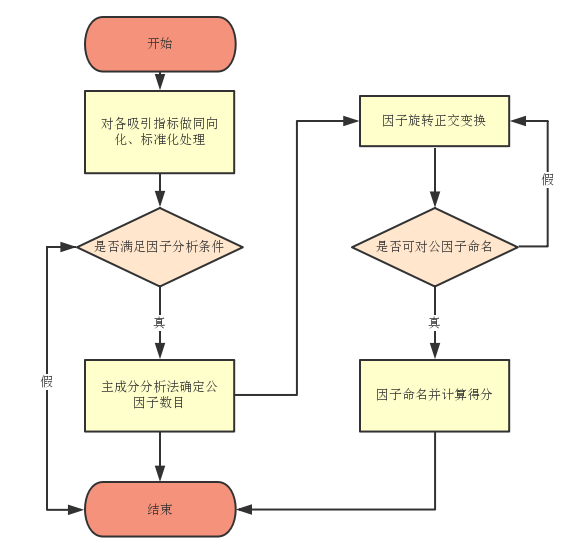
\includegraphics[width=\textwidth]{figures/1111.png}
		\caption{因子分析算法流程图}\label{llll}
	\end{figure}

		\subsection{预备工作}
		\subsubsection{评价指标体系构建}
		参考国家统计局对人才标准的划分,此处对人才的界 定是指,具有大专及以上学历的人员,以及具有初级以上 专业技术职称的人员或在专业技术岗位上工作的人员。
		
		在构建武汉市人才吸引力评价指标体系时,在指标方面,若选取总量太多,在评价模型时太为复杂,可行性低,若数据太少则评价不够准确,脱离实际性。因此为尽可能客观反映吸引力,我们在遵循建立指标体系的科学性、系统性、可操作性、可比性原则\parencite{lepawsky2010metropolis},并兼顾总量指标和相对指标,选取城市发展前景、主要行业收入、政府影响、环境因素、年末总人口共5个二级指标和33个三级指标,多维度、全方面的考虑各个指标对人才吸引力的影响。具体指标体系如图~\ref{lct}~所示: 	
		\begin{figure}[H]
			\centering
			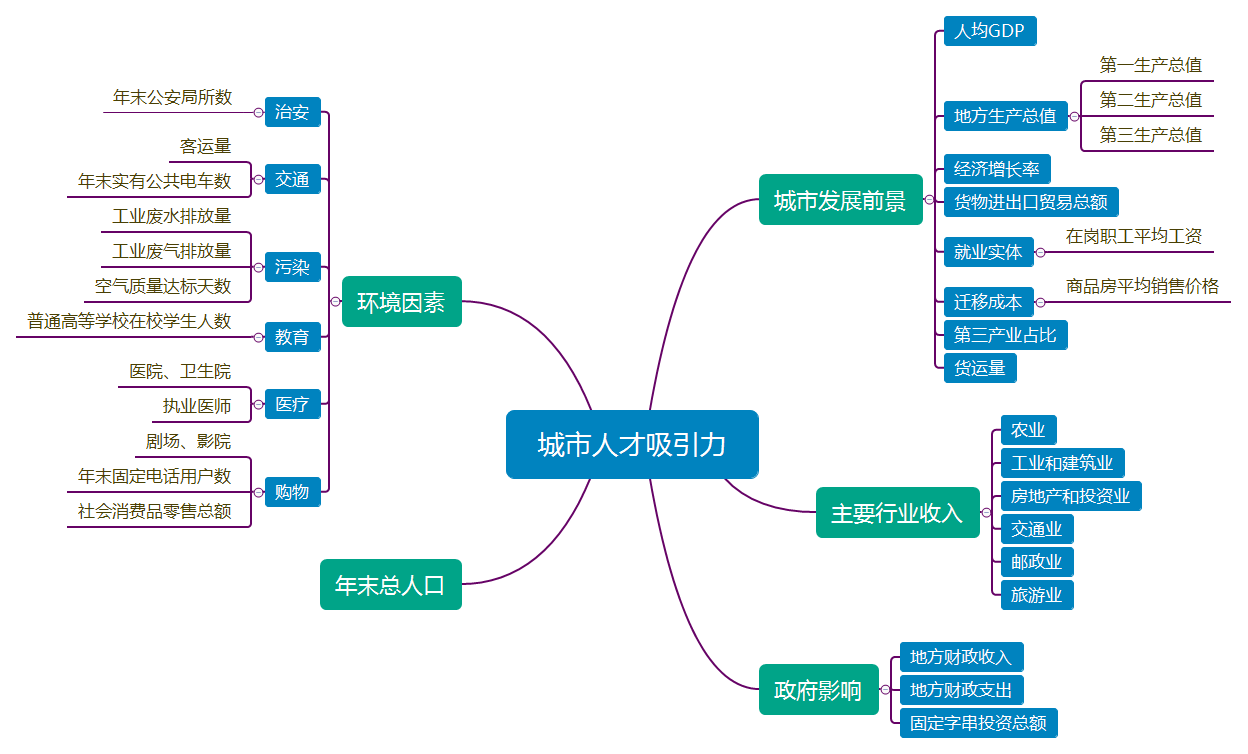
\includegraphics[width=\textwidth]{figures/clt.png}
			\caption{城市人才吸引力指标体系}\label{lct}
		\end{figure}  
		
		\subsubsection{同向化处理}

		在评价城市人才的指标中,工业废水废气排放量和商品房平均销售价格不是越高越好,为方便比较,对这三个指标进行同向化处理\parencite{张瑞红2012河南省产业集群环境人才吸引力评价研究}, 其公式如下:
		\begin{gather}
		\widetilde{X}=-(X-\overline{X})
		\end{gather}
		式中:$X$原始指标,$\overline{X}$为原始指标$X$的平均值,$\widetilde{X}$为同向化指标。
		
		\subsubsection{标准化处理}
		为了对变量进行比较并消除由于观测量纲的差异及数量级差异所造成的影响,将样本观测数据进行标准化处理,使标准化的变量均值为$0$,方差为$1$。其处理方法如下:
		\begin{gather}
		Z=\frac{X-\overline{X}}{\delta_{X}}
		\end{gather}
		式中:$\overline{X}$为$X$的均值,$\delta_{X}$是$X$的标准差。
		
		\subsubsection{KMO与Bartlett检验}
		根据标准化处理后的指标数据,利用$SPSS23.0$统计软件进行$KMO$和巴特利特检验,以确认所选变量是否适合做因子分析,结果如表\label{tab1}所示:
		% Table generated by Excel2LaTeX from sheet 'Sheet1'
		\begin{table}[H]
			\centering
			\caption{KMO和Bartlett的检验}\label{tab1}
			\begin{tabular}{cc|cc|cc}
				\toprule[1.5pt]
				\multicolumn{4}{c|}{取样足够度的Kaiser-Meyer-Olkin度量} & \multicolumn{2}{c}{0.859} \\
				\midrule
				\multicolumn{2}{c|}{\multirow{3}[2]{*}{Bartlett的球形度检验}} & \multicolumn{2}{c|}{近似卡方} & \multicolumn{2}{c}{1183.981} \\
				\multicolumn{2}{c|}{} & \multicolumn{2}{c|}{df} & \multicolumn{2}{c}{78} \\
				\multicolumn{2}{c|}{} & \multicolumn{2}{c|}{Sig.} & \multicolumn{2}{c}{.000} \\
				\bottomrule[2pt]
			\end{tabular}%
			\label{tab:addlabel}%
		\end{table}%
		
		由上表可知,巴特利特球度检验统计量的观测值为$1183.981$,相应的概率$P$值接近$0$。若显著性水平$α$为$0.5$,概率$P$小于显著性水平$α$,应拒绝零假设,认为相关系数矩阵与单位阵有显著差异,即因子协方差矩阵不是单位阵。同时,$KMO$值为$0.859$,$KMO>0.8$,根据$KMO$ 度量标准可知原有变量适合进行因子分析。
		
		
		

	\subsection{模型的建立与求解}
	\subsubsection{公因子的确定}
	根据上述指标标准化后,其对应相关系数矩阵部分数据见表~\ref{shuju2}~所示(详见附件~\ref{shuju}~):
	%三线表
	\begin{table}[H]
		 \centering
		\caption{相关系数矩阵部分数据}\label{shuju2}
		\begin{tabular}{ccccccc}
			\toprule[2pt]
			\multicolumn{1}{m{1cm}}{\centering } &
			\multicolumn{1}{m{2cm}}{\centering $X_{1}$} & \multicolumn{1}{m{2cm}}{\centering $X_{2}$} & \multicolumn{1}{m{2cm}}{\centering $X_{3}$}&
			\multicolumn{1}{m{2cm}}{\centering $X_{4}$}&
			\multicolumn{1}{m{1cm}}{\centering ........} &
			\multicolumn{1}{m{2cm}}{\centering $X_{33}$}
			\\
				\midrule[1pt]
			$X_{1}$&1.000	 &  0.727 & -0.423&0.967&........& -0.928\\ 
			$X_{2}$& &  1.000 & -0.796&0.822&........&-0.814\\ 
			$X_{3}$& &   & 1.000&-0.620&........&0.682\\ 
			$X_{4}$& &   & &1.000&........&-0.955\\ 
			........& &   & & &........&........\\ 
			$X_{33}$& &   & & &........&1.000\\
			\bottomrule[2pt]
		\end{tabular}
	\end{table}
	
	设$\lambda_{1} \geqslant \lambda_{2} \geqslant \cdots \geqslant \lambda_{p}$为样本相关系数矩阵$R$的特征值,$\eta _ { 1 } , \eta _ { 2 } , \cdots , n _ { p }$为相应的标准正交化特征向量。设$m<p$,则因子载荷矩阵$\Lambda$为:
	\begin{gather}
	\Lambda=\left[\sqrt{\lambda_{1}} \eta_{1}, \sqrt{\lambda_{2}} \eta_{2}, \cdots, \sqrt{\lambda_{m}} \eta_{m}\right]
	\end{gather}
    用$\boldsymbol{R}-\boldsymbol{\Lambda} \boldsymbol{\Lambda}^{\mathrm{T}}$对角元来估计特殊因子的的方差:
	\begin{gather}
	\sigma_{i}^{2}=1-\sum_{j=1}^{m} \alpha_{i j}^{2}
	\end{gather}
	式中:$\sigma_{i}^{2}$为方差,$\alpha_{i j}^{2}$表示载荷因子。由上述分析,得总方差解释部分数据如表~\ref{biaosan}~所示:	
		\begin{table}[H]
		\centering
		\caption{总方差解释}\label{biaosan}
		\begin{tabular}{ccccccc}
			\toprule[1.5pt]
		\multicolumn{1}{m{1cm}}{\centering } &
				\multicolumn{1}{m{1.5cm}}{\centering  } &
		 \multicolumn{1}{m{3cm}}{\centering 初始特征值} &
		 		\multicolumn{1}{m{1cm}}{\centering  } &
		\multicolumn{1}{m{1cm}}{\centering  } &
		 \multicolumn{1}{m{3cm}}{\centering 提取载荷平方和}&
		 		\multicolumn{1}{m{1.5cm}}{\centering  } \\\hline
		\multicolumn{1}{m{1cm}}{\centering  成分} &
		\multicolumn{1}{m{1.5cm}}{\centering  总计} &
		\multicolumn{1}{m{2cm}}{\centering  方差百分比} &
		\multicolumn{1}{m{1cm}}{\centering  累积} &
		\multicolumn{1}{m{1cm}}{\centering  总计} &
		\multicolumn{1}{m{3cm}}{\centering  方差百分比} &				\multicolumn{1}{m{1.5cm}}{\centering  累积} \\

			\midrule[1pt]
			0&25.330&76.758&76.758&25.330&76.758&76.758 \\
			1&4.025&12.197&88.956&4.025&12.197&88.956 \\
			2&2.373&7.191&96.147&2.373&7.191&96.147 \\
			3&1.271&3.852&99.920&1.271&3.852&99.920 \\
			4&5.129e-15&1.554e-14&100.0&&& \\
			5&1.330e-15&4.031e-15&100.0&&& \\
			6&6.062e-16&1.837e-15&100.0&&& \\
			7&5.067e-16&1.535e-15&100.0&&& \\
			8&4.532e-16&1.373e-15&100.0&&& \\
			9&3.335e-16&1.011e-15&100.0&&& \\
			10&3.137e-16&9.506e-16&100.0&&& \\
			11&2.585e-16&7.834e-16&100.0&&& \\
			12&1.990e-16&6.031e-16&100.0&&& \\
			......&......&.......&100.0&&& \\
			......&......&.......&100.0&&& \\
			33&-2.279e-15&-6.908e-15&100.0&&& \\
			\bottomrule[1.5pt]
		\end{tabular}
	\end{table}
	
	
	由表~\ref{biaosan}~特征根知,因子$F_{1}$的特征值$\lambda_{1}=25.330$,占方差的 $76.75\%$。由碎石图~\ref{123}~可知,当提取$1,2$个公因子时,特征值变化非常明显,当提取第$5$个以后的公因子时,特征值变化比较小,基本趋于平缓。由此说明,提取$4$个公因子对原变量信息的刻画有显著作用。因此,在这里我们提取$4$个公共因子,这$4$个公因子的累计方差达到$99.92\%$,即这$4$个公因子可以反映原来$33$个指标的$99.92\%$的信息量,可见采用前\textbf{4个公因子}对武汉2013——2017年人才吸引力进行评价是比较合适的。
	
	\begin{figure}[H]
		\centering
		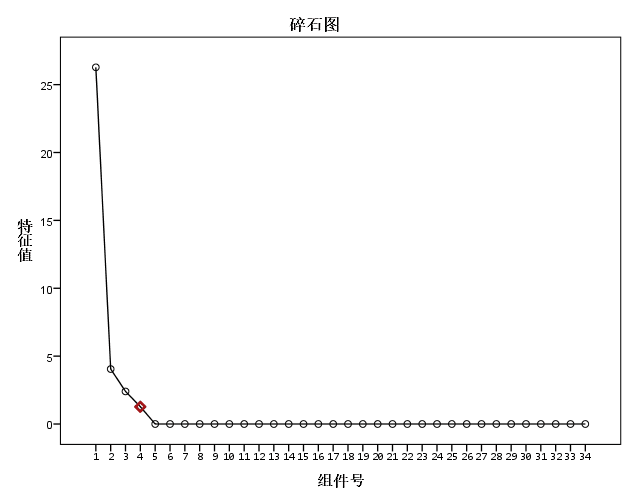
\includegraphics[width=\textwidth]{figures/123.png}
		\caption{碎石图}\label{123}
	\end{figure} 
	
	\subsubsection{未转轴的因子载荷矩阵}

	表~\ref{cehngfenjuzheng}~(详见附录)是初始因子载荷矩阵,由此可写出因子分析模型的如下:
	\begin{gather}
	\begin{array} { l } { \mathrm { X } _ { 1 } = 0.989 \mathrm { F } _ { 1 } + 0.123 \mathrm { F } _ { 2 } - 0.074 \mathrm { F } _ { 3 } - 0.031 \mathrm { F } _ { 4 } } \\ { \mathrm { X } _ { 2 } = 0.795 \mathrm { F } _ { 1 } - 0.556 \mathrm { F } _ { 2 } - 0.193 \mathrm { F } _ { 3 } - 0.151 \mathrm { F } _ { 4 } } \\ { \ldots \ldots } \\ { \mathrm { X } _ { 33 } = - 0.958 \mathrm { F } _ { 1 } + 0.176 \mathrm { F } _ { 2 } - 0.060 \mathrm { F } _ { 3 } + 0.220 \mathrm { F } _ { 4 } } \end{array}
	\end{gather}
		表~\ref{cehngfenjuzheng}~中的每个数据表示了相应因子变量对相应原变量的相对重要程度。由于得到的公共因子与各指标的载荷分布归类比较困难,需要对因子载荷矩阵进行正交旋转,这里运用方差最大正交旋转法\parencite{宋鸿2010城市人才吸引力的影响因素及提升对策},得到旋转后的因子载荷矩阵表~\ref{xuanzhuanhuo}~所示。
		
		
		
	根据表~\ref{xuanzhuanhuo}~发现,通过最大正交旋转法,旋转在\textbf{9次迭代}后已收敛。旋转后的因子系数已经明显向两极分化,有了更鲜明的实际意义。因子载荷的绝对值越大,则表明该因子与变量的重叠性越高,在解释因子的时候就越重要。
	(因子命名)
	
	
	\subsubsection{求得因子得分和综合绩效得分}
	采用回归法估计因子得分系数,并输出因子得分系数矩阵。具体结果见表$6$
	由估计出的因子得分,可以量化描述城市人才吸引力水平,利用因子得分可以从不同角度对城市人才吸引力水平进行比较分析。为了便于对各城市进行人才吸引力评价,现利用武汉每年度的因子得分表计算综合得分,吸引力水平的获取是基于总方差分解表中旋转后各因子的方差贡献率及计算所得的城市各因子得分获取的。其计算公式如下:
	\begin{gather}
	\mathrm { F } = \left( 55.267 \mathrm { F } _ { 1 } + 17.845 \mathrm { F } _ { 2 } + 14.623 \mathrm { F } _ { 3 } + 12.265 \mathrm { F } _ { 4 } \right) / 99.92
	%(附结果计算公式)
	\end{gather}
	计算结果见表$7$
	\subsection{结果分析}
	
	\section{问题二模型的建立与求解}
	\subsection{问题的描述与分析}
	问题二要求针对具体人才类别,


%	\parencite{geng2019novel}为文献引用
	查阅资料可得\parencite{宋鸿2010城市人才吸引力的影响因素及提升对策}
	
%	~\ref{llllll}~为图表引用,中间为为图表\label{}
具体浓度分布如图~\ref{llllll}~所示:


	\section{问题二模型的建立与求解}
	\subsection{问题的描述与分析}
%	问题分析写\textbf{流程图!!}其流程图如图~\ref{lct}~所示:
%			\begin{figure}[H]
%	\centering
%	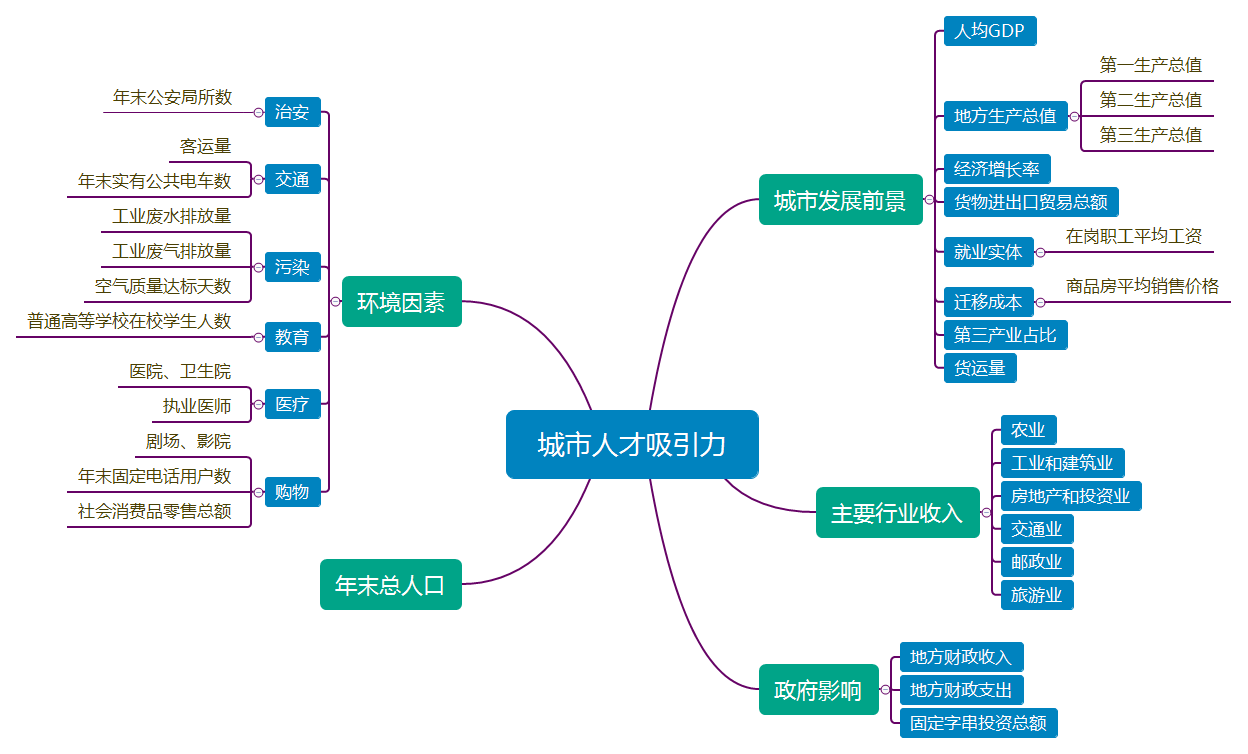
\includegraphics[width=.8\textwidth]{figures/clt.png}
%	\caption{算法流程图}\label{lct}
%	\end{figure}
	\subsection{模型的建立与求解}
	

	\section{问题三模型的建立与求解}
	
	
	\subsection{问题的描述与分析}

	\subsection{模型的建立与求解}


	\section{模型的评价}
	\subsection{模型的优点}
xxxxxxxxxxxxxxxxxxxxxxxxx
	
	\subsection{模型的缺点}
xxxxxxxxxxxxxxxxxxxxxxxxxxxxxx


	\subsection{模型的改进与展望}%
xxxxxxxxxxxxxxxxxxxxxxxxxxxx
	\newpage	%换页符
	%%参考文献
	%\begin{thebibliography}{9}%宽度9
	% \setlength{\itemsep}{-2mm}
	\nocite{*}		%排版未引用的参考文献
	\printbibliography[title = {参考文献}]	%使用国标参考文献添加方式
	%参考文献添加到wenxian.bib里,再引用
	
	\newpage
	%附录
	\appendix %%附录
\section{代码}
\subsection{爬取数据--python源代码}
\begin{lstlisting}[language=python]%这里修改语言
xxxxxxxxxxxxxxxxxxxxxxxxxxxxxxxx
\end{lstlisting}

\subsection{相关系数矩阵}
% Table generated by Excel2LaTeX from sheet 'Sheet1'
\begin{table}[H]
	\centering
	\caption{33个指标的相关系数矩阵}
	\begin{tabular}{r|r|r|r|r|r|r|r|r|r|r|r|r|r|r|r|r|r|r|r|r|r|r|r|r|r|r|r|r|r|r|r|r}
		\hline
		\textcolor[rgb]{ .004,  .008,  .02}{1.000} & \textcolor[rgb]{ .004,  .008,  .02}{0.727} & \textcolor[rgb]{ .004,  .008,  .02}{-0.423} & \textcolor[rgb]{ .004,  .008,  .02}{0.967} & \textcolor[rgb]{ .004,  .008,  .02}{0.973} & \textcolor[rgb]{ .004,  .008,  .02}{0.937} & \textcolor[rgb]{ .004,  .008,  .02}{0.799} & \textcolor[rgb]{ .004,  .008,  .02}{0.989} & \textcolor[rgb]{ .004,  .008,  .02}{0.989} & \textcolor[rgb]{ .004,  .008,  .02}{-0.988} & \textcolor[rgb]{ .004,  .008,  .02}{0.994} & \textcolor[rgb]{ .004,  .008,  .02}{0.969} & \textcolor[rgb]{ .004,  .008,  .02}{0.960} & \textcolor[rgb]{ .004,  .008,  .02}{0.797} & \textcolor[rgb]{ .004,  .008,  .02}{0.898} & \textcolor[rgb]{ .004,  .008,  .02}{0.246} & \textcolor[rgb]{ .004,  .008,  .02}{-0.670} & \textcolor[rgb]{ .004,  .008,  .02}{-0.898} & \textcolor[rgb]{ .004,  .008,  .02}{0.614} & \textcolor[rgb]{ .004,  .008,  .02}{-0.119} & \textcolor[rgb]{ .004,  .008,  .02}{0.914} & \textcolor[rgb]{ .004,  .008,  .02}{-0.927} & \textcolor[rgb]{ .004,  .008,  .02}{0.985} & \textcolor[rgb]{ .004,  .008,  .02}{0.991} & \textcolor[rgb]{ .004,  .008,  .02}{0.513} & \textcolor[rgb]{ .004,  .008,  .02}{0.766} & \textcolor[rgb]{ .004,  .008,  .02}{0.967} & \textcolor[rgb]{ .004,  .008,  .02}{-0.963} & \textcolor[rgb]{ .004,  .008,  .02}{0.984} & \textcolor[rgb]{ .004,  .008,  .02}{0.954} & \textcolor[rgb]{ .004,  .008,  .02}{0.973} & \textcolor[rgb]{ .004,  .008,  .02}{0.881} & \textcolor[rgb]{ .004,  .008,  .02}{-0.928} \bigstrut\\
		\hline
		\textcolor[rgb]{ .004,  .008,  .02}{0.727} & \textcolor[rgb]{ .004,  .008,  .02}{1.000} & \textcolor[rgb]{ .004,  .008,  .02}{-0.796} & \textcolor[rgb]{ .004,  .008,  .02}{0.822} & \textcolor[rgb]{ .004,  .008,  .02}{0.832} & \textcolor[rgb]{ .004,  .008,  .02}{0.721} & \textcolor[rgb]{ .004,  .008,  .02}{0.760} & \textcolor[rgb]{ .004,  .008,  .02}{0.707} & \textcolor[rgb]{ .004,  .008,  .02}{0.802} & \textcolor[rgb]{ .004,  .008,  .02}{-0.657} & \textcolor[rgb]{ .004,  .008,  .02}{0.716} & \textcolor[rgb]{ .004,  .008,  .02}{0.746} & \textcolor[rgb]{ .004,  .008,  .02}{0.785} & \textcolor[rgb]{ .004,  .008,  .02}{0.318} & \textcolor[rgb]{ .004,  .008,  .02}{0.465} & \textcolor[rgb]{ .004,  .008,  .02}{-0.478} & \textcolor[rgb]{ .004,  .008,  .02}{-0.615} & \textcolor[rgb]{ .004,  .008,  .02}{-0.674} & \textcolor[rgb]{ .004,  .008,  .02}{0.436} & \textcolor[rgb]{ .004,  .008,  .02}{-0.603} & \textcolor[rgb]{ .004,  .008,  .02}{0.422} & \textcolor[rgb]{ .004,  .008,  .02}{-0.690} & \textcolor[rgb]{ .004,  .008,  .02}{0.813} & \textcolor[rgb]{ .004,  .008,  .02}{0.793} & \textcolor[rgb]{ .004,  .008,  .02}{0.930} & \textcolor[rgb]{ .004,  .008,  .02}{0.762} & \textcolor[rgb]{ .004,  .008,  .02}{0.699} & \textcolor[rgb]{ .004,  .008,  .02}{-0.737} & \textcolor[rgb]{ .004,  .008,  .02}{0.814} & \textcolor[rgb]{ .004,  .008,  .02}{0.582} & \textcolor[rgb]{ .004,  .008,  .02}{0.816} & \textcolor[rgb]{ .004,  .008,  .02}{0.881} & \textcolor[rgb]{ .004,  .008,  .02}{-0.814} \bigstrut\\
		\hline
		\textcolor[rgb]{ .004,  .008,  .02}{-0.423} & \textcolor[rgb]{ .004,  .008,  .02}{-0.796} & \textcolor[rgb]{ .004,  .008,  .02}{1.000} & \textcolor[rgb]{ .004,  .008,  .02}{-0.620} & \textcolor[rgb]{ .004,  .008,  .02}{-0.470} & \textcolor[rgb]{ .004,  .008,  .02}{-0.293} & \textcolor[rgb]{ .004,  .008,  .02}{-0.825} & \textcolor[rgb]{ .004,  .008,  .02}{-0.469} & \textcolor[rgb]{ .004,  .008,  .02}{-0.518} & \textcolor[rgb]{ .004,  .008,  .02}{0.311} & \textcolor[rgb]{ .004,  .008,  .02}{-0.357} & \textcolor[rgb]{ .004,  .008,  .02}{-0.586} & \textcolor[rgb]{ .004,  .008,  .02}{-0.629} & \textcolor[rgb]{ .004,  .008,  .02}{0.034} & \textcolor[rgb]{ .004,  .008,  .02}{-0.179} & \textcolor[rgb]{ .004,  .008,  .02}{0.493} & \textcolor[rgb]{ .004,  .008,  .02}{0.016} & \textcolor[rgb]{ .004,  .008,  .02}{0.164} & \textcolor[rgb]{ .004,  .008,  .02}{-0.428} & \textcolor[rgb]{ .004,  .008,  .02}{0.873} & \textcolor[rgb]{ .004,  .008,  .02}{-0.213} & \textcolor[rgb]{ .004,  .008,  .02}{0.597} & \textcolor[rgb]{ .004,  .008,  .02}{-0.569} & \textcolor[rgb]{ .004,  .008,  .02}{-0.529} & \textcolor[rgb]{ .004,  .008,  .02}{-0.674} & \textcolor[rgb]{ .004,  .008,  .02}{-0.758} & \textcolor[rgb]{ .004,  .008,  .02}{-0.534} & \textcolor[rgb]{ .004,  .008,  .02}{0.593} & \textcolor[rgb]{ .004,  .008,  .02}{-0.561} & \textcolor[rgb]{ .004,  .008,  .02}{-0.424} & \textcolor[rgb]{ .004,  .008,  .02}{-0.493} & \textcolor[rgb]{ .004,  .008,  .02}{-0.689} & \textcolor[rgb]{ .004,  .008,  .02}{0.682} \bigstrut\\
		\hline
		\textcolor[rgb]{ .004,  .008,  .02}{0.967} & \textcolor[rgb]{ .004,  .008,  .02}{0.822} & \textcolor[rgb]{ .004,  .008,  .02}{-0.620} & \textcolor[rgb]{ .004,  .008,  .02}{1.000} & \textcolor[rgb]{ .004,  .008,  .02}{0.947} & \textcolor[rgb]{ .004,  .008,  .02}{0.853} & \textcolor[rgb]{ .004,  .008,  .02}{0.909} & \textcolor[rgb]{ .004,  .008,  .02}{0.961} & \textcolor[rgb]{ .004,  .008,  .02}{0.973} & \textcolor[rgb]{ .004,  .008,  .02}{-0.919} & \textcolor[rgb]{ .004,  .008,  .02}{0.941} & \textcolor[rgb]{ .004,  .008,  .02}{0.985} & \textcolor[rgb]{ .004,  .008,  .02}{0.996} & \textcolor[rgb]{ .004,  .008,  .02}{0.720} & \textcolor[rgb]{ .004,  .008,  .02}{0.854} & \textcolor[rgb]{ .004,  .008,  .02}{0.094} & \textcolor[rgb]{ .004,  .008,  .02}{-0.578} & \textcolor[rgb]{ .004,  .008,  .02}{-0.797} & \textcolor[rgb]{ .004,  .008,  .02}{0.713} & \textcolor[rgb]{ .004,  .008,  .02}{-0.285} & \textcolor[rgb]{ .004,  .008,  .02}{0.831} & \textcolor[rgb]{ .004,  .008,  .02}{-0.970} & \textcolor[rgb]{ .004,  .008,  .02}{0.995} & \textcolor[rgb]{ .004,  .008,  .02}{0.982} & \textcolor[rgb]{ .004,  .008,  .02}{0.585} & \textcolor[rgb]{ .004,  .008,  .02}{0.895} & \textcolor[rgb]{ .004,  .008,  .02}{0.981} & \textcolor[rgb]{ .004,  .008,  .02}{-0.985} & \textcolor[rgb]{ .004,  .008,  .02}{0.980} & \textcolor[rgb]{ .004,  .008,  .02}{0.927} & \textcolor[rgb]{ .004,  .008,  .02}{0.944} & \textcolor[rgb]{ .004,  .008,  .02}{0.961} & \textcolor[rgb]{ .004,  .008,  .02}{-0.955} \bigstrut\\
		\hline
		\textcolor[rgb]{ .004,  .008,  .02}{0.973} & \textcolor[rgb]{ .004,  .008,  .02}{0.832} & \textcolor[rgb]{ .004,  .008,  .02}{-0.470} & \textcolor[rgb]{ .004,  .008,  .02}{0.947} & \textcolor[rgb]{ .004,  .008,  .02}{1.000} & \textcolor[rgb]{ .004,  .008,  .02}{0.969} & \textcolor[rgb]{ .004,  .008,  .02}{0.752} & \textcolor[rgb]{ .004,  .008,  .02}{0.951} & \textcolor[rgb]{ .004,  .008,  .02}{0.986} & \textcolor[rgb]{ .004,  .008,  .02}{-0.961} & \textcolor[rgb]{ .004,  .008,  .02}{0.981} & \textcolor[rgb]{ .004,  .008,  .02}{0.925} & \textcolor[rgb]{ .004,  .008,  .02}{0.922} & \textcolor[rgb]{ .004,  .008,  .02}{0.704} & \textcolor[rgb]{ .004,  .008,  .02}{0.806} & \textcolor[rgb]{ .004,  .008,  .02}{0.048} & \textcolor[rgb]{ .004,  .008,  .02}{-0.771} & \textcolor[rgb]{ .004,  .008,  .02}{-0.940} & \textcolor[rgb]{ .004,  .008,  .02}{0.512} & \textcolor[rgb]{ .004,  .008,  .02}{-0.211} & \textcolor[rgb]{ .004,  .008,  .02}{0.816} & \textcolor[rgb]{ .004,  .008,  .02}{-0.854} & \textcolor[rgb]{ .004,  .008,  .02}{0.971} & \textcolor[rgb]{ .004,  .008,  .02}{0.979} & \textcolor[rgb]{ .004,  .008,  .02}{0.685} & \textcolor[rgb]{ .004,  .008,  .02}{0.726} & \textcolor[rgb]{ .004,  .008,  .02}{0.905} & \textcolor[rgb]{ .004,  .008,  .02}{-0.912} & \textcolor[rgb]{ .004,  .008,  .02}{0.978} & \textcolor[rgb]{ .004,  .008,  .02}{0.872} & \textcolor[rgb]{ .004,  .008,  .02}{0.992} & \textcolor[rgb]{ .004,  .008,  .02}{0.889} & \textcolor[rgb]{ .004,  .008,  .02}{-0.918} \bigstrut\\
		\hline
		\textcolor[rgb]{ .004,  .008,  .02}{0.937} & \textcolor[rgb]{ .004,  .008,  .02}{0.721} & \textcolor[rgb]{ .004,  .008,  .02}{-0.293} & \textcolor[rgb]{ .004,  .008,  .02}{0.853} & \textcolor[rgb]{ .004,  .008,  .02}{0.969} & \textcolor[rgb]{ .004,  .008,  .02}{1.000} & \textcolor[rgb]{ .004,  .008,  .02}{0.608} & \textcolor[rgb]{ .004,  .008,  .02}{0.919} & \textcolor[rgb]{ .004,  .008,  .02}{0.947} & \textcolor[rgb]{ .004,  .008,  .02}{-0.962} & \textcolor[rgb]{ .004,  .008,  .02}{0.965} & \textcolor[rgb]{ .004,  .008,  .02}{0.851} & \textcolor[rgb]{ .004,  .008,  .02}{0.827} & \textcolor[rgb]{ .004,  .008,  .02}{0.671} & \textcolor[rgb]{ .004,  .008,  .02}{0.750} & \textcolor[rgb]{ .004,  .008,  .02}{0.142} & \textcolor[rgb]{ .004,  .008,  .02}{-0.801} & \textcolor[rgb]{ .004,  .008,  .02}{-0.978} & \textcolor[rgb]{ .004,  .008,  .02}{0.326} & \textcolor[rgb]{ .004,  .008,  .02}{-0.114} & \textcolor[rgb]{ .004,  .008,  .02}{0.832} & \textcolor[rgb]{ .004,  .008,  .02}{-0.745} & \textcolor[rgb]{ .004,  .008,  .02}{0.899} & \textcolor[rgb]{ .004,  .008,  .02}{0.930} & \textcolor[rgb]{ .004,  .008,  .02}{0.624} & \textcolor[rgb]{ .004,  .008,  .02}{0.540} & \textcolor[rgb]{ .004,  .008,  .02}{0.822} & \textcolor[rgb]{ .004,  .008,  .02}{-0.830} & \textcolor[rgb]{ .004,  .008,  .02}{0.928} & \textcolor[rgb]{ .004,  .008,  .02}{0.835} & \textcolor[rgb]{ .004,  .008,  .02}{0.971} & \textcolor[rgb]{ .004,  .008,  .02}{0.748} & \textcolor[rgb]{ .004,  .008,  .02}{-0.855} \bigstrut\\
		\hline
		\textcolor[rgb]{ .004,  .008,  .02}{0.799} & \textcolor[rgb]{ .004,  .008,  .02}{0.760} & \textcolor[rgb]{ .004,  .008,  .02}{-0.825} & \textcolor[rgb]{ .004,  .008,  .02}{0.909} & \textcolor[rgb]{ .004,  .008,  .02}{0.752} & \textcolor[rgb]{ .004,  .008,  .02}{0.608} & \textcolor[rgb]{ .004,  .008,  .02}{1.000} & \textcolor[rgb]{ .004,  .008,  .02}{0.838} & \textcolor[rgb]{ .004,  .008,  .02}{0.828} & \textcolor[rgb]{ .004,  .008,  .02}{-0.718} & \textcolor[rgb]{ .004,  .008,  .02}{0.735} & \textcolor[rgb]{ .004,  .008,  .02}{0.917} & \textcolor[rgb]{ .004,  .008,  .02}{0.933} & \textcolor[rgb]{ .004,  .008,  .02}{0.473} & \textcolor[rgb]{ .004,  .008,  .02}{0.665} & \textcolor[rgb]{ .004,  .008,  .02}{0.025} & \textcolor[rgb]{ .004,  .008,  .02}{-0.208} & \textcolor[rgb]{ .004,  .008,  .02}{-0.489} & \textcolor[rgb]{ .004,  .008,  .02}{0.712} & \textcolor[rgb]{ .004,  .008,  .02}{-0.537} & \textcolor[rgb]{ .004,  .008,  .02}{0.702} & \textcolor[rgb]{ .004,  .008,  .02}{-0.939} & \textcolor[rgb]{ .004,  .008,  .02}{0.876} & \textcolor[rgb]{ .004,  .008,  .02}{0.849} & \textcolor[rgb]{ .004,  .008,  .02}{0.493} & \textcolor[rgb]{ .004,  .008,  .02}{0.933} & \textcolor[rgb]{ .004,  .008,  .02}{0.903} & \textcolor[rgb]{ .004,  .008,  .02}{-0.926} & \textcolor[rgb]{ .004,  .008,  .02}{0.858} & \textcolor[rgb]{ .004,  .008,  .02}{0.846} & \textcolor[rgb]{ .004,  .008,  .02}{0.777} & \textcolor[rgb]{ .004,  .008,  .02}{0.881} & \textcolor[rgb]{ .004,  .008,  .02}{-0.919} \bigstrut\\
		\hline
		\textcolor[rgb]{ .004,  .008,  .02}{0.989} & \textcolor[rgb]{ .004,  .008,  .02}{0.707} & \textcolor[rgb]{ .004,  .008,  .02}{-0.469} & \textcolor[rgb]{ .004,  .008,  .02}{0.961} & \textcolor[rgb]{ .004,  .008,  .02}{0.951} & \textcolor[rgb]{ .004,  .008,  .02}{0.919} & \textcolor[rgb]{ .004,  .008,  .02}{0.838} & \textcolor[rgb]{ .004,  .008,  .02}{1.000} & \textcolor[rgb]{ .004,  .008,  .02}{0.987} & \textcolor[rgb]{ .004,  .008,  .02}{-0.979} & \textcolor[rgb]{ .004,  .008,  .02}{0.976} & \textcolor[rgb]{ .004,  .008,  .02}{0.985} & \textcolor[rgb]{ .004,  .008,  .02}{0.965} & \textcolor[rgb]{ .004,  .008,  .02}{0.731} & \textcolor[rgb]{ .004,  .008,  .02}{0.858} & \textcolor[rgb]{ .004,  .008,  .02}{0.279} & \textcolor[rgb]{ .004,  .008,  .02}{-0.570} & \textcolor[rgb]{ .004,  .008,  .02}{-0.850} & \textcolor[rgb]{ .004,  .008,  .02}{0.573} & \textcolor[rgb]{ .004,  .008,  .02}{-0.201} & \textcolor[rgb]{ .004,  .008,  .02}{0.939} & \textcolor[rgb]{ .004,  .008,  .02}{-0.937} & \textcolor[rgb]{ .004,  .008,  .02}{0.978} & \textcolor[rgb]{ .004,  .008,  .02}{0.990} & \textcolor[rgb]{ .004,  .008,  .02}{0.486} & \textcolor[rgb]{ .004,  .008,  .02}{0.757} & \textcolor[rgb]{ .004,  .008,  .02}{0.972} & \textcolor[rgb]{ .004,  .008,  .02}{-0.977} & \textcolor[rgb]{ .004,  .008,  .02}{0.986} & \textcolor[rgb]{ .004,  .008,  .02}{0.979} & \textcolor[rgb]{ .004,  .008,  .02}{0.969} & \textcolor[rgb]{ .004,  .008,  .02}{0.850} & \textcolor[rgb]{ .004,  .008,  .02}{-0.960} \bigstrut\\
		\hline
		\textcolor[rgb]{ .004,  .008,  .02}{0.989} & \textcolor[rgb]{ .004,  .008,  .02}{0.802} & \textcolor[rgb]{ .004,  .008,  .02}{-0.518} & \textcolor[rgb]{ .004,  .008,  .02}{0.973} & \textcolor[rgb]{ .004,  .008,  .02}{0.986} & \textcolor[rgb]{ .004,  .008,  .02}{0.947} & \textcolor[rgb]{ .004,  .008,  .02}{0.828} & \textcolor[rgb]{ .004,  .008,  .02}{0.987} & \textcolor[rgb]{ .004,  .008,  .02}{1.000} & \textcolor[rgb]{ .004,  .008,  .02}{-0.973} & \textcolor[rgb]{ .004,  .008,  .02}{0.982} & \textcolor[rgb]{ .004,  .008,  .02}{0.972} & \textcolor[rgb]{ .004,  .008,  .02}{0.963} & \textcolor[rgb]{ .004,  .008,  .02}{0.700} & \textcolor[rgb]{ .004,  .008,  .02}{0.826} & \textcolor[rgb]{ .004,  .008,  .02}{0.134} & \textcolor[rgb]{ .004,  .008,  .02}{-0.659} & \textcolor[rgb]{ .004,  .008,  .02}{-0.891} & \textcolor[rgb]{ .004,  .008,  .02}{0.551} & \textcolor[rgb]{ .004,  .008,  .02}{-0.254} & \textcolor[rgb]{ .004,  .008,  .02}{0.876} & \textcolor[rgb]{ .004,  .008,  .02}{-0.913} & \textcolor[rgb]{ .004,  .008,  .02}{0.990} & \textcolor[rgb]{ .004,  .008,  .02}{0.999} & \textcolor[rgb]{ .004,  .008,  .02}{0.615} & \textcolor[rgb]{ .004,  .008,  .02}{0.769} & \textcolor[rgb]{ .004,  .008,  .02}{0.952} & \textcolor[rgb]{ .004,  .008,  .02}{-0.962} & \textcolor[rgb]{ .004,  .008,  .02}{0.998} & \textcolor[rgb]{ .004,  .008,  .02}{0.935} & \textcolor[rgb]{ .004,  .008,  .02}{0.993} & \textcolor[rgb]{ .004,  .008,  .02}{0.891} & \textcolor[rgb]{ .004,  .008,  .02}{-0.963} \bigstrut\\
		\hline
		\textcolor[rgb]{ .004,  .008,  .02}{-0.988} & \textcolor[rgb]{ .004,  .008,  .02}{-0.657} & \textcolor[rgb]{ .004,  .008,  .02}{0.311} & \textcolor[rgb]{ .004,  .008,  .02}{-0.919} & \textcolor[rgb]{ .004,  .008,  .02}{-0.961} & \textcolor[rgb]{ .004,  .008,  .02}{-0.962} & \textcolor[rgb]{ .004,  .008,  .02}{-0.718} & \textcolor[rgb]{ .004,  .008,  .02}{-0.979} & \textcolor[rgb]{ .004,  .008,  .02}{-0.973} & \textcolor[rgb]{ .004,  .008,  .02}{1.000} & \textcolor[rgb]{ .004,  .008,  .02}{-0.995} & \textcolor[rgb]{ .004,  .008,  .02}{-0.935} & \textcolor[rgb]{ .004,  .008,  .02}{-0.911} & \textcolor[rgb]{ .004,  .008,  .02}{-0.794} & \textcolor[rgb]{ .004,  .008,  .02}{-0.881} & \textcolor[rgb]{ .004,  .008,  .02}{-0.321} & \textcolor[rgb]{ .004,  .008,  .02}{0.691} & \textcolor[rgb]{ .004,  .008,  .02}{0.928} & \textcolor[rgb]{ .004,  .008,  .02}{-0.515} & \textcolor[rgb]{ .004,  .008,  .02}{0.048} & \textcolor[rgb]{ .004,  .008,  .02}{-0.938} & \textcolor[rgb]{ .004,  .008,  .02}{0.872} & \textcolor[rgb]{ .004,  .008,  .02}{-0.950} & \textcolor[rgb]{ .004,  .008,  .02}{-0.970} & \textcolor[rgb]{ .004,  .008,  .02}{-0.467} & \textcolor[rgb]{ .004,  .008,  .02}{-0.662} & \textcolor[rgb]{ .004,  .008,  .02}{-0.929} & \textcolor[rgb]{ .004,  .008,  .02}{0.924} & \textcolor[rgb]{ .004,  .008,  .02}{-0.961} & \textcolor[rgb]{ .004,  .008,  .02}{-0.945} & \textcolor[rgb]{ .004,  .008,  .02}{-0.967} & \textcolor[rgb]{ .004,  .008,  .02}{-0.802} & \textcolor[rgb]{ .004,  .008,  .02}{0.896} \bigstrut\\
		\hline
		\textcolor[rgb]{ .004,  .008,  .02}{0.994} & \textcolor[rgb]{ .004,  .008,  .02}{0.716} & \textcolor[rgb]{ .004,  .008,  .02}{-0.357} & \textcolor[rgb]{ .004,  .008,  .02}{0.941} & \textcolor[rgb]{ .004,  .008,  .02}{0.981} & \textcolor[rgb]{ .004,  .008,  .02}{0.965} & \textcolor[rgb]{ .004,  .008,  .02}{0.735} & \textcolor[rgb]{ .004,  .008,  .02}{0.976} & \textcolor[rgb]{ .004,  .008,  .02}{0.982} & \textcolor[rgb]{ .004,  .008,  .02}{-0.995} & \textcolor[rgb]{ .004,  .008,  .02}{1.000} & \textcolor[rgb]{ .004,  .008,  .02}{0.940} & \textcolor[rgb]{ .004,  .008,  .02}{0.926} & \textcolor[rgb]{ .004,  .008,  .02}{0.798} & \textcolor[rgb]{ .004,  .008,  .02}{0.885} & \textcolor[rgb]{ .004,  .008,  .02}{0.241} & \textcolor[rgb]{ .004,  .008,  .02}{-0.732} & \textcolor[rgb]{ .004,  .008,  .02}{-0.939} & \textcolor[rgb]{ .004,  .008,  .02}{0.553} & \textcolor[rgb]{ .004,  .008,  .02}{-0.073} & \textcolor[rgb]{ .004,  .008,  .02}{0.904} & \textcolor[rgb]{ .004,  .008,  .02}{-0.882} & \textcolor[rgb]{ .004,  .008,  .02}{0.967} & \textcolor[rgb]{ .004,  .008,  .02}{0.980} & \textcolor[rgb]{ .004,  .008,  .02}{0.529} & \textcolor[rgb]{ .004,  .008,  .02}{0.705} & \textcolor[rgb]{ .004,  .008,  .02}{0.935} & \textcolor[rgb]{ .004,  .008,  .02}{-0.930} & \textcolor[rgb]{ .004,  .008,  .02}{0.972} & \textcolor[rgb]{ .004,  .008,  .02}{0.928} & \textcolor[rgb]{ .004,  .008,  .02}{0.977} & \textcolor[rgb]{ .004,  .008,  .02}{0.850} & \textcolor[rgb]{ .004,  .008,  .02}{-0.901} \bigstrut\\
		\hline
		\textcolor[rgb]{ .004,  .008,  .02}{0.969} & \textcolor[rgb]{ .004,  .008,  .02}{0.746} & \textcolor[rgb]{ .004,  .008,  .02}{-0.586} & \textcolor[rgb]{ .004,  .008,  .02}{0.985} & \textcolor[rgb]{ .004,  .008,  .02}{0.925} & \textcolor[rgb]{ .004,  .008,  .02}{0.851} & \textcolor[rgb]{ .004,  .008,  .02}{0.917} & \textcolor[rgb]{ .004,  .008,  .02}{0.985} & \textcolor[rgb]{ .004,  .008,  .02}{0.972} & \textcolor[rgb]{ .004,  .008,  .02}{-0.935} & \textcolor[rgb]{ .004,  .008,  .02}{0.940} & \textcolor[rgb]{ .004,  .008,  .02}{1.000} & \textcolor[rgb]{ .004,  .008,  .02}{0.994} & \textcolor[rgb]{ .004,  .008,  .02}{0.705} & \textcolor[rgb]{ .004,  .008,  .02}{0.851} & \textcolor[rgb]{ .004,  .008,  .02}{0.217} & \textcolor[rgb]{ .004,  .008,  .02}{-0.491} & \textcolor[rgb]{ .004,  .008,  .02}{-0.772} & \textcolor[rgb]{ .004,  .008,  .02}{0.668} & \textcolor[rgb]{ .004,  .008,  .02}{-0.283} & \textcolor[rgb]{ .004,  .008,  .02}{0.899} & \textcolor[rgb]{ .004,  .008,  .02}{-0.979} & \textcolor[rgb]{ .004,  .008,  .02}{0.985} & \textcolor[rgb]{ .004,  .008,  .02}{0.982} & \textcolor[rgb]{ .004,  .008,  .02}{0.495} & \textcolor[rgb]{ .004,  .008,  .02}{0.854} & \textcolor[rgb]{ .004,  .008,  .02}{0.992} & \textcolor[rgb]{ .004,  .008,  .02}{-0.999} & \textcolor[rgb]{ .004,  .008,  .02}{0.981} & \textcolor[rgb]{ .004,  .008,  .02}{0.973} & \textcolor[rgb]{ .004,  .008,  .02}{0.940} & \textcolor[rgb]{ .004,  .008,  .02}{0.902} & \textcolor[rgb]{ .004,  .008,  .02}{-0.974} \bigstrut\\
		\hline
		\textcolor[rgb]{ .004,  .008,  .02}{0.960} & \textcolor[rgb]{ .004,  .008,  .02}{0.785} & \textcolor[rgb]{ .004,  .008,  .02}{-0.629} & \textcolor[rgb]{ .004,  .008,  .02}{0.996} & \textcolor[rgb]{ .004,  .008,  .02}{0.922} & \textcolor[rgb]{ .004,  .008,  .02}{0.827} & \textcolor[rgb]{ .004,  .008,  .02}{0.933} & \textcolor[rgb]{ .004,  .008,  .02}{0.965} & \textcolor[rgb]{ .004,  .008,  .02}{0.963} & \textcolor[rgb]{ .004,  .008,  .02}{-0.911} & \textcolor[rgb]{ .004,  .008,  .02}{0.926} & \textcolor[rgb]{ .004,  .008,  .02}{0.994} & \textcolor[rgb]{ .004,  .008,  .02}{1.000} & \textcolor[rgb]{ .004,  .008,  .02}{0.709} & \textcolor[rgb]{ .004,  .008,  .02}{0.853} & \textcolor[rgb]{ .004,  .008,  .02}{0.148} & \textcolor[rgb]{ .004,  .008,  .02}{-0.505} & \textcolor[rgb]{ .004,  .008,  .02}{-0.756} & \textcolor[rgb]{ .004,  .008,  .02}{0.722} & \textcolor[rgb]{ .004,  .008,  .02}{-0.298} & \textcolor[rgb]{ .004,  .008,  .02}{0.854} & \textcolor[rgb]{ .004,  .008,  .02}{-0.986} & \textcolor[rgb]{ .004,  .008,  .02}{0.988} & \textcolor[rgb]{ .004,  .008,  .02}{0.975} & \textcolor[rgb]{ .004,  .008,  .02}{0.530} & \textcolor[rgb]{ .004,  .008,  .02}{0.901} & \textcolor[rgb]{ .004,  .008,  .02}{0.991} & \textcolor[rgb]{ .004,  .008,  .02}{-0.996} & \textcolor[rgb]{ .004,  .008,  .02}{0.974} & \textcolor[rgb]{ .004,  .008,  .02}{0.948} & \textcolor[rgb]{ .004,  .008,  .02}{0.928} & \textcolor[rgb]{ .004,  .008,  .02}{0.942} & \textcolor[rgb]{ .004,  .008,  .02}{-0.963} \bigstrut\\
		\hline
		\textcolor[rgb]{ .004,  .008,  .02}{0.797} & \textcolor[rgb]{ .004,  .008,  .02}{0.318} & \textcolor[rgb]{ .004,  .008,  .02}{0.034} & \textcolor[rgb]{ .004,  .008,  .02}{0.720} & \textcolor[rgb]{ .004,  .008,  .02}{0.704} & \textcolor[rgb]{ .004,  .008,  .02}{0.671} & \textcolor[rgb]{ .004,  .008,  .02}{0.473} & \textcolor[rgb]{ .004,  .008,  .02}{0.731} & \textcolor[rgb]{ .004,  .008,  .02}{0.700} & \textcolor[rgb]{ .004,  .008,  .02}{-0.794} & \textcolor[rgb]{ .004,  .008,  .02}{0.798} & \textcolor[rgb]{ .004,  .008,  .02}{0.705} & \textcolor[rgb]{ .004,  .008,  .02}{0.709} & \textcolor[rgb]{ .004,  .008,  .02}{1.000} & \textcolor[rgb]{ .004,  .008,  .02}{0.971} & \textcolor[rgb]{ .004,  .008,  .02}{0.522} & \textcolor[rgb]{ .004,  .008,  .02}{-0.632} & \textcolor[rgb]{ .004,  .008,  .02}{-0.733} & \textcolor[rgb]{ .004,  .008,  .02}{0.751} & \textcolor[rgb]{ .004,  .008,  .02}{0.456} & \textcolor[rgb]{ .004,  .008,  .02}{0.776} & \textcolor[rgb]{ .004,  .008,  .02}{-0.742} & \textcolor[rgb]{ .004,  .008,  .02}{0.730} & \textcolor[rgb]{ .004,  .008,  .02}{0.717} & \textcolor[rgb]{ .004,  .008,  .02}{0.062} & \textcolor[rgb]{ .004,  .008,  .02}{0.604} & \textcolor[rgb]{ .004,  .008,  .02}{0.777} & \textcolor[rgb]{ .004,  .008,  .02}{-0.715} & \textcolor[rgb]{ .004,  .008,  .02}{0.681} & \textcolor[rgb]{ .004,  .008,  .02}{0.754} & \textcolor[rgb]{ .004,  .008,  .02}{0.656} & \textcolor[rgb]{ .004,  .008,  .02}{0.675} & \textcolor[rgb]{ .004,  .008,  .02}{-0.539} \bigstrut\\
		\hline
		\textcolor[rgb]{ .004,  .008,  .02}{0.898} & \textcolor[rgb]{ .004,  .008,  .02}{0.465} & \textcolor[rgb]{ .004,  .008,  .02}{-0.179} & \textcolor[rgb]{ .004,  .008,  .02}{0.854} & \textcolor[rgb]{ .004,  .008,  .02}{0.806} & \textcolor[rgb]{ .004,  .008,  .02}{0.750} & \textcolor[rgb]{ .004,  .008,  .02}{0.665} & \textcolor[rgb]{ .004,  .008,  .02}{0.858} & \textcolor[rgb]{ .004,  .008,  .02}{0.826} & \textcolor[rgb]{ .004,  .008,  .02}{-0.881} & \textcolor[rgb]{ .004,  .008,  .02}{0.885} & \textcolor[rgb]{ .004,  .008,  .02}{0.851} & \textcolor[rgb]{ .004,  .008,  .02}{0.853} & \textcolor[rgb]{ .004,  .008,  .02}{0.971} & \textcolor[rgb]{ .004,  .008,  .02}{1.000} & \textcolor[rgb]{ .004,  .008,  .02}{0.473} & \textcolor[rgb]{ .004,  .008,  .02}{-0.591} & \textcolor[rgb]{ .004,  .008,  .02}{-0.766} & \textcolor[rgb]{ .004,  .008,  .02}{0.800} & \textcolor[rgb]{ .004,  .008,  .02}{0.241} & \textcolor[rgb]{ .004,  .008,  .02}{0.868} & \textcolor[rgb]{ .004,  .008,  .02}{-0.880} & \textcolor[rgb]{ .004,  .008,  .02}{0.857} & \textcolor[rgb]{ .004,  .008,  .02}{0.844} & \textcolor[rgb]{ .004,  .008,  .02}{0.180} & \textcolor[rgb]{ .004,  .008,  .02}{0.743} & \textcolor[rgb]{ .004,  .008,  .02}{0.904} & \textcolor[rgb]{ .004,  .008,  .02}{-0.860} & \textcolor[rgb]{ .004,  .008,  .02}{0.817} & \textcolor[rgb]{ .004,  .008,  .02}{0.880} & \textcolor[rgb]{ .004,  .008,  .02}{0.777} & \textcolor[rgb]{ .004,  .008,  .02}{0.795} & \textcolor[rgb]{ .004,  .008,  .02}{-0.714} \bigstrut\\
		\hline
		\textcolor[rgb]{ .004,  .008,  .02}{0.246} & \textcolor[rgb]{ .004,  .008,  .02}{-0.478} & \textcolor[rgb]{ .004,  .008,  .02}{0.493} & \textcolor[rgb]{ .004,  .008,  .02}{0.094} & \textcolor[rgb]{ .004,  .008,  .02}{0.048} & \textcolor[rgb]{ .004,  .008,  .02}{0.142} & \textcolor[rgb]{ .004,  .008,  .02}{0.025} & \textcolor[rgb]{ .004,  .008,  .02}{0.279} & \textcolor[rgb]{ .004,  .008,  .02}{0.134} & \textcolor[rgb]{ .004,  .008,  .02}{-0.321} & \textcolor[rgb]{ .004,  .008,  .02}{0.241} & \textcolor[rgb]{ .004,  .008,  .02}{0.217} & \textcolor[rgb]{ .004,  .008,  .02}{0.148} & \textcolor[rgb]{ .004,  .008,  .02}{0.522} & \textcolor[rgb]{ .004,  .008,  .02}{0.473} & \textcolor[rgb]{ .004,  .008,  .02}{1.000} & \textcolor[rgb]{ .004,  .008,  .02}{0.122} & \textcolor[rgb]{ .004,  .008,  .02}{-0.131} & \textcolor[rgb]{ .004,  .008,  .02}{0.196} & \textcolor[rgb]{ .004,  .008,  .02}{0.606} & \textcolor[rgb]{ .004,  .008,  .02}{0.588} & \textcolor[rgb]{ .004,  .008,  .02}{-0.252} & \textcolor[rgb]{ .004,  .008,  .02}{0.120} & \textcolor[rgb]{ .004,  .008,  .02}{0.154} & \textcolor[rgb]{ .004,  .008,  .02}{-0.679} & \textcolor[rgb]{ .004,  .008,  .02}{-0.047} & \textcolor[rgb]{ .004,  .008,  .02}{0.277} & \textcolor[rgb]{ .004,  .008,  .02}{-0.224} & \textcolor[rgb]{ .004,  .008,  .02}{0.118} & \textcolor[rgb]{ .004,  .008,  .02}{0.429} & \textcolor[rgb]{ .004,  .008,  .02}{0.084} & \textcolor[rgb]{ .004,  .008,  .02}{-0.108} & \textcolor[rgb]{ .004,  .008,  .02}{-0.077} \bigstrut\\
		\hline
		\textcolor[rgb]{ .004,  .008,  .02}{-0.670} & \textcolor[rgb]{ .004,  .008,  .02}{-0.615} & \textcolor[rgb]{ .004,  .008,  .02}{0.016} & \textcolor[rgb]{ .004,  .008,  .02}{-0.578} & \textcolor[rgb]{ .004,  .008,  .02}{-0.771} & \textcolor[rgb]{ .004,  .008,  .02}{-0.801} & \textcolor[rgb]{ .004,  .008,  .02}{-0.208} & \textcolor[rgb]{ .004,  .008,  .02}{-0.570} & \textcolor[rgb]{ .004,  .008,  .02}{-0.659} & \textcolor[rgb]{ .004,  .008,  .02}{0.691} & \textcolor[rgb]{ .004,  .008,  .02}{-0.732} & \textcolor[rgb]{ .004,  .008,  .02}{-0.491} & \textcolor[rgb]{ .004,  .008,  .02}{-0.505} & \textcolor[rgb]{ .004,  .008,  .02}{-0.632} & \textcolor[rgb]{ .004,  .008,  .02}{-0.591} & \textcolor[rgb]{ .004,  .008,  .02}{0.122} & \textcolor[rgb]{ .004,  .008,  .02}{1.000} & \textcolor[rgb]{ .004,  .008,  .02}{0.900} & \textcolor[rgb]{ .004,  .008,  .02}{-0.247} & \textcolor[rgb]{ .004,  .008,  .02}{-0.182} & \textcolor[rgb]{ .004,  .008,  .02}{-0.433} & \textcolor[rgb]{ .004,  .008,  .02}{0.402} & \textcolor[rgb]{ .004,  .008,  .02}{-0.624} & \textcolor[rgb]{ .004,  .008,  .02}{-0.635} & \textcolor[rgb]{ .004,  .008,  .02}{-0.632} & \textcolor[rgb]{ .004,  .008,  .02}{-0.325} & \textcolor[rgb]{ .004,  .008,  .02}{-0.492} & \textcolor[rgb]{ .004,  .008,  .02}{0.472} & \textcolor[rgb]{ .004,  .008,  .02}{-0.624} & \textcolor[rgb]{ .004,  .008,  .02}{-0.430} & \textcolor[rgb]{ .004,  .008,  .02}{-0.706} & \textcolor[rgb]{ .004,  .008,  .02}{-0.598} & \textcolor[rgb]{ .004,  .008,  .02}{0.459} \bigstrut\\
		\hline
		\textcolor[rgb]{ .004,  .008,  .02}{-0.898} & \textcolor[rgb]{ .004,  .008,  .02}{-0.674} & \textcolor[rgb]{ .004,  .008,  .02}{0.164} & \textcolor[rgb]{ .004,  .008,  .02}{-0.797} & \textcolor[rgb]{ .004,  .008,  .02}{-0.940} & \textcolor[rgb]{ .004,  .008,  .02}{-0.978} & \textcolor[rgb]{ .004,  .008,  .02}{-0.489} & \textcolor[rgb]{ .004,  .008,  .02}{-0.850} & \textcolor[rgb]{ .004,  .008,  .02}{-0.891} & \textcolor[rgb]{ .004,  .008,  .02}{0.928} & \textcolor[rgb]{ .004,  .008,  .02}{-0.939} & \textcolor[rgb]{ .004,  .008,  .02}{-0.772} & \textcolor[rgb]{ .004,  .008,  .02}{-0.756} & \textcolor[rgb]{ .004,  .008,  .02}{-0.733} & \textcolor[rgb]{ .004,  .008,  .02}{-0.766} & \textcolor[rgb]{ .004,  .008,  .02}{-0.131} & \textcolor[rgb]{ .004,  .008,  .02}{0.900} & \textcolor[rgb]{ .004,  .008,  .02}{1.000} & \textcolor[rgb]{ .004,  .008,  .02}{-0.336} & \textcolor[rgb]{ .004,  .008,  .02}{-0.044} & \textcolor[rgb]{ .004,  .008,  .02}{-0.766} & \textcolor[rgb]{ .004,  .008,  .02}{0.673} & \textcolor[rgb]{ .004,  .008,  .02}{-0.846} & \textcolor[rgb]{ .004,  .008,  .02}{-0.873} & \textcolor[rgb]{ .004,  .008,  .02}{-0.597} & \textcolor[rgb]{ .004,  .008,  .02}{-0.485} & \textcolor[rgb]{ .004,  .008,  .02}{-0.759} & \textcolor[rgb]{ .004,  .008,  .02}{0.752} & \textcolor[rgb]{ .004,  .008,  .02}{-0.864} & \textcolor[rgb]{ .004,  .008,  .02}{-0.755} & \textcolor[rgb]{ .004,  .008,  .02}{-0.920} & \textcolor[rgb]{ .004,  .008,  .02}{-0.720} & \textcolor[rgb]{ .004,  .008,  .02}{0.750} \bigstrut\\
		\hline
		\textcolor[rgb]{ .004,  .008,  .02}{0.614} & \textcolor[rgb]{ .004,  .008,  .02}{0.436} & \textcolor[rgb]{ .004,  .008,  .02}{-0.428} & \textcolor[rgb]{ .004,  .008,  .02}{0.713} & \textcolor[rgb]{ .004,  .008,  .02}{0.512} & \textcolor[rgb]{ .004,  .008,  .02}{0.326} & \textcolor[rgb]{ .004,  .008,  .02}{0.712} & \textcolor[rgb]{ .004,  .008,  .02}{0.573} & \textcolor[rgb]{ .004,  .008,  .02}{0.551} & \textcolor[rgb]{ .004,  .008,  .02}{-0.515} & \textcolor[rgb]{ .004,  .008,  .02}{0.553} & \textcolor[rgb]{ .004,  .008,  .02}{0.668} & \textcolor[rgb]{ .004,  .008,  .02}{0.722} & \textcolor[rgb]{ .004,  .008,  .02}{0.751} & \textcolor[rgb]{ .004,  .008,  .02}{0.800} & \textcolor[rgb]{ .004,  .008,  .02}{0.196} & \textcolor[rgb]{ .004,  .008,  .02}{-0.247} & \textcolor[rgb]{ .004,  .008,  .02}{-0.336} & \textcolor[rgb]{ .004,  .008,  .02}{1.000} & \textcolor[rgb]{ .004,  .008,  .02}{0.060} & \textcolor[rgb]{ .004,  .008,  .02}{0.510} & \textcolor[rgb]{ .004,  .008,  .02}{-0.797} & \textcolor[rgb]{ .004,  .008,  .02}{0.657} & \textcolor[rgb]{ .004,  .008,  .02}{0.591} & \textcolor[rgb]{ .004,  .008,  .02}{0.105} & \textcolor[rgb]{ .004,  .008,  .02}{0.887} & \textcolor[rgb]{ .004,  .008,  .02}{0.744} & \textcolor[rgb]{ .004,  .008,  .02}{-0.700} & \textcolor[rgb]{ .004,  .008,  .02}{0.569} & \textcolor[rgb]{ .004,  .008,  .02}{0.625} & \textcolor[rgb]{ .004,  .008,  .02}{0.463} & \textcolor[rgb]{ .004,  .008,  .02}{0.786} & \textcolor[rgb]{ .004,  .008,  .02}{-0.521} \bigstrut\\
		\hline
		\textcolor[rgb]{ .004,  .008,  .02}{-0.119} & \textcolor[rgb]{ .004,  .008,  .02}{-0.603} & \textcolor[rgb]{ .004,  .008,  .02}{0.873} & \textcolor[rgb]{ .004,  .008,  .02}{-0.285} & \textcolor[rgb]{ .004,  .008,  .02}{-0.211} & \textcolor[rgb]{ .004,  .008,  .02}{-0.114} & \textcolor[rgb]{ .004,  .008,  .02}{-0.537} & \textcolor[rgb]{ .004,  .008,  .02}{-0.201} & \textcolor[rgb]{ .004,  .008,  .02}{-0.254} & \textcolor[rgb]{ .004,  .008,  .02}{0.048} & \textcolor[rgb]{ .004,  .008,  .02}{-0.073} & \textcolor[rgb]{ .004,  .008,  .02}{-0.283} & \textcolor[rgb]{ .004,  .008,  .02}{-0.298} & \textcolor[rgb]{ .004,  .008,  .02}{0.456} & \textcolor[rgb]{ .004,  .008,  .02}{0.241} & \textcolor[rgb]{ .004,  .008,  .02}{0.606} & \textcolor[rgb]{ .004,  .008,  .02}{-0.182} & \textcolor[rgb]{ .004,  .008,  .02}{-0.044} & \textcolor[rgb]{ .004,  .008,  .02}{0.060} & \textcolor[rgb]{ .004,  .008,  .02}{1.000} & \textcolor[rgb]{ .004,  .008,  .02}{0.031} & \textcolor[rgb]{ .004,  .008,  .02}{0.233} & \textcolor[rgb]{ .004,  .008,  .02}{-0.257} & \textcolor[rgb]{ .004,  .008,  .02}{-0.248} & \textcolor[rgb]{ .004,  .008,  .02}{-0.632} & \textcolor[rgb]{ .004,  .008,  .02}{-0.356} & \textcolor[rgb]{ .004,  .008,  .02}{-0.186} & \textcolor[rgb]{ .004,  .008,  .02}{0.274} & \textcolor[rgb]{ .004,  .008,  .02}{-0.295} & \textcolor[rgb]{ .004,  .008,  .02}{-0.137} & \textcolor[rgb]{ .004,  .008,  .02}{-0.269} & \textcolor[rgb]{ .004,  .008,  .02}{-0.313} & \textcolor[rgb]{ .004,  .008,  .02}{0.465} \bigstrut\\
		\hline
		\textcolor[rgb]{ .004,  .008,  .02}{0.914} & \textcolor[rgb]{ .004,  .008,  .02}{0.422} & \textcolor[rgb]{ .004,  .008,  .02}{-0.213} & \textcolor[rgb]{ .004,  .008,  .02}{0.831} & \textcolor[rgb]{ .004,  .008,  .02}{0.816} & \textcolor[rgb]{ .004,  .008,  .02}{0.832} & \textcolor[rgb]{ .004,  .008,  .02}{0.702} & \textcolor[rgb]{ .004,  .008,  .02}{0.939} & \textcolor[rgb]{ .004,  .008,  .02}{0.876} & \textcolor[rgb]{ .004,  .008,  .02}{-0.938} & \textcolor[rgb]{ .004,  .008,  .02}{0.904} & \textcolor[rgb]{ .004,  .008,  .02}{0.899} & \textcolor[rgb]{ .004,  .008,  .02}{0.854} & \textcolor[rgb]{ .004,  .008,  .02}{0.776} & \textcolor[rgb]{ .004,  .008,  .02}{0.868} & \textcolor[rgb]{ .004,  .008,  .02}{0.588} & \textcolor[rgb]{ .004,  .008,  .02}{-0.433} & \textcolor[rgb]{ .004,  .008,  .02}{-0.766} & \textcolor[rgb]{ .004,  .008,  .02}{0.510} & \textcolor[rgb]{ .004,  .008,  .02}{0.031} & \textcolor[rgb]{ .004,  .008,  .02}{1.000} & \textcolor[rgb]{ .004,  .008,  .02}{-0.862} & \textcolor[rgb]{ .004,  .008,  .02}{0.858} & \textcolor[rgb]{ .004,  .008,  .02}{0.884} & \textcolor[rgb]{ .004,  .008,  .02}{0.176} & \textcolor[rgb]{ .004,  .008,  .02}{0.593} & \textcolor[rgb]{ .004,  .008,  .02}{0.904} & \textcolor[rgb]{ .004,  .008,  .02}{-0.893} & \textcolor[rgb]{ .004,  .008,  .02}{0.870} & \textcolor[rgb]{ .004,  .008,  .02}{0.972} & \textcolor[rgb]{ .004,  .008,  .02}{0.848} & \textcolor[rgb]{ .004,  .008,  .02}{0.656} & \textcolor[rgb]{ .004,  .008,  .02}{-0.837} \bigstrut\\
		\hline
		\textcolor[rgb]{ .004,  .008,  .02}{-0.927} & \textcolor[rgb]{ .004,  .008,  .02}{-0.690} & \textcolor[rgb]{ .004,  .008,  .02}{0.597} & \textcolor[rgb]{ .004,  .008,  .02}{-0.970} & \textcolor[rgb]{ .004,  .008,  .02}{-0.854} & \textcolor[rgb]{ .004,  .008,  .02}{-0.745} & \textcolor[rgb]{ .004,  .008,  .02}{-0.939} & \textcolor[rgb]{ .004,  .008,  .02}{-0.937} & \textcolor[rgb]{ .004,  .008,  .02}{-0.913} & \textcolor[rgb]{ .004,  .008,  .02}{0.872} & \textcolor[rgb]{ .004,  .008,  .02}{-0.882} & \textcolor[rgb]{ .004,  .008,  .02}{-0.979} & \textcolor[rgb]{ .004,  .008,  .02}{-0.986} & \textcolor[rgb]{ .004,  .008,  .02}{-0.742} & \textcolor[rgb]{ .004,  .008,  .02}{-0.880} & \textcolor[rgb]{ .004,  .008,  .02}{-0.252} & \textcolor[rgb]{ .004,  .008,  .02}{0.402} & \textcolor[rgb]{ .004,  .008,  .02}{0.673} & \textcolor[rgb]{ .004,  .008,  .02}{-0.797} & \textcolor[rgb]{ .004,  .008,  .02}{0.233} & \textcolor[rgb]{ .004,  .008,  .02}{-0.862} & \textcolor[rgb]{ .004,  .008,  .02}{1.000} & \textcolor[rgb]{ .004,  .008,  .02}{-0.953} & \textcolor[rgb]{ .004,  .008,  .02}{-0.934} & \textcolor[rgb]{ .004,  .008,  .02}{-0.392} & \textcolor[rgb]{ .004,  .008,  .02}{-0.919} & \textcolor[rgb]{ .004,  .008,  .02}{-0.991} & \textcolor[rgb]{ .004,  .008,  .02}{0.988} & \textcolor[rgb]{ .004,  .008,  .02}{-0.927} & \textcolor[rgb]{ .004,  .008,  .02}{-0.953} & \textcolor[rgb]{ .004,  .008,  .02}{-0.861} & \textcolor[rgb]{ .004,  .008,  .02}{-0.914} & \textcolor[rgb]{ .004,  .008,  .02}{0.921} \bigstrut\\
		\hline
		\textcolor[rgb]{ .004,  .008,  .02}{0.985} & \textcolor[rgb]{ .004,  .008,  .02}{0.813} & \textcolor[rgb]{ .004,  .008,  .02}{-0.569} & \textcolor[rgb]{ .004,  .008,  .02}{0.995} & \textcolor[rgb]{ .004,  .008,  .02}{0.971} & \textcolor[rgb]{ .004,  .008,  .02}{0.899} & \textcolor[rgb]{ .004,  .008,  .02}{0.876} & \textcolor[rgb]{ .004,  .008,  .02}{0.978} & \textcolor[rgb]{ .004,  .008,  .02}{0.990} & \textcolor[rgb]{ .004,  .008,  .02}{-0.950} & \textcolor[rgb]{ .004,  .008,  .02}{0.967} & \textcolor[rgb]{ .004,  .008,  .02}{0.985} & \textcolor[rgb]{ .004,  .008,  .02}{0.988} & \textcolor[rgb]{ .004,  .008,  .02}{0.730} & \textcolor[rgb]{ .004,  .008,  .02}{0.857} & \textcolor[rgb]{ .004,  .008,  .02}{0.120} & \textcolor[rgb]{ .004,  .008,  .02}{-0.624} & \textcolor[rgb]{ .004,  .008,  .02}{-0.846} & \textcolor[rgb]{ .004,  .008,  .02}{0.657} & \textcolor[rgb]{ .004,  .008,  .02}{-0.257} & \textcolor[rgb]{ .004,  .008,  .02}{0.858} & \textcolor[rgb]{ .004,  .008,  .02}{-0.953} & \textcolor[rgb]{ .004,  .008,  .02}{1.000} & \textcolor[rgb]{ .004,  .008,  .02}{0.995} & \textcolor[rgb]{ .004,  .008,  .02}{0.594} & \textcolor[rgb]{ .004,  .008,  .02}{0.848} & \textcolor[rgb]{ .004,  .008,  .02}{0.977} & \textcolor[rgb]{ .004,  .008,  .02}{-0.982} & \textcolor[rgb]{ .004,  .008,  .02}{0.993} & \textcolor[rgb]{ .004,  .008,  .02}{0.937} & \textcolor[rgb]{ .004,  .008,  .02}{0.970} & \textcolor[rgb]{ .004,  .008,  .02}{0.939} & \textcolor[rgb]{ .004,  .008,  .02}{-0.960} \bigstrut\\
		\hline
		\textcolor[rgb]{ .004,  .008,  .02}{0.991} & \textcolor[rgb]{ .004,  .008,  .02}{0.793} & \textcolor[rgb]{ .004,  .008,  .02}{-0.529} & \textcolor[rgb]{ .004,  .008,  .02}{0.982} & \textcolor[rgb]{ .004,  .008,  .02}{0.979} & \textcolor[rgb]{ .004,  .008,  .02}{0.930} & \textcolor[rgb]{ .004,  .008,  .02}{0.849} & \textcolor[rgb]{ .004,  .008,  .02}{0.990} & \textcolor[rgb]{ .004,  .008,  .02}{0.999} & \textcolor[rgb]{ .004,  .008,  .02}{-0.970} & \textcolor[rgb]{ .004,  .008,  .02}{0.980} & \textcolor[rgb]{ .004,  .008,  .02}{0.982} & \textcolor[rgb]{ .004,  .008,  .02}{0.975} & \textcolor[rgb]{ .004,  .008,  .02}{0.717} & \textcolor[rgb]{ .004,  .008,  .02}{0.844} & \textcolor[rgb]{ .004,  .008,  .02}{0.154} & \textcolor[rgb]{ .004,  .008,  .02}{-0.635} & \textcolor[rgb]{ .004,  .008,  .02}{-0.873} & \textcolor[rgb]{ .004,  .008,  .02}{0.591} & \textcolor[rgb]{ .004,  .008,  .02}{-0.248} & \textcolor[rgb]{ .004,  .008,  .02}{0.884} & \textcolor[rgb]{ .004,  .008,  .02}{-0.934} & \textcolor[rgb]{ .004,  .008,  .02}{0.995} & \textcolor[rgb]{ .004,  .008,  .02}{1.000} & \textcolor[rgb]{ .004,  .008,  .02}{0.589} & \textcolor[rgb]{ .004,  .008,  .02}{0.796} & \textcolor[rgb]{ .004,  .008,  .02}{0.967} & \textcolor[rgb]{ .004,  .008,  .02}{-0.975} & \textcolor[rgb]{ .004,  .008,  .02}{0.999} & \textcolor[rgb]{ .004,  .008,  .02}{0.947} & \textcolor[rgb]{ .004,  .008,  .02}{0.986} & \textcolor[rgb]{ .004,  .008,  .02}{0.903} & \textcolor[rgb]{ .004,  .008,  .02}{-0.966} \bigstrut\\
		\hline
		\textcolor[rgb]{ .004,  .008,  .02}{0.513} & \textcolor[rgb]{ .004,  .008,  .02}{0.930} & \textcolor[rgb]{ .004,  .008,  .02}{-0.674} & \textcolor[rgb]{ .004,  .008,  .02}{0.585} & \textcolor[rgb]{ .004,  .008,  .02}{0.685} & \textcolor[rgb]{ .004,  .008,  .02}{0.624} & \textcolor[rgb]{ .004,  .008,  .02}{0.493} & \textcolor[rgb]{ .004,  .008,  .02}{0.486} & \textcolor[rgb]{ .004,  .008,  .02}{0.615} & \textcolor[rgb]{ .004,  .008,  .02}{-0.467} & \textcolor[rgb]{ .004,  .008,  .02}{0.529} & \textcolor[rgb]{ .004,  .008,  .02}{0.495} & \textcolor[rgb]{ .004,  .008,  .02}{0.530} & \textcolor[rgb]{ .004,  .008,  .02}{0.062} & \textcolor[rgb]{ .004,  .008,  .02}{0.180} & \textcolor[rgb]{ .004,  .008,  .02}{-0.679} & \textcolor[rgb]{ .004,  .008,  .02}{-0.632} & \textcolor[rgb]{ .004,  .008,  .02}{-0.597} & \textcolor[rgb]{ .004,  .008,  .02}{0.105} & \textcolor[rgb]{ .004,  .008,  .02}{-0.632} & \textcolor[rgb]{ .004,  .008,  .02}{0.176} & \textcolor[rgb]{ .004,  .008,  .02}{-0.392} & \textcolor[rgb]{ .004,  .008,  .02}{0.594} & \textcolor[rgb]{ .004,  .008,  .02}{0.589} & \textcolor[rgb]{ .004,  .008,  .02}{1.000} & \textcolor[rgb]{ .004,  .008,  .02}{0.477} & \textcolor[rgb]{ .004,  .008,  .02}{0.422} & \textcolor[rgb]{ .004,  .008,  .02}{-0.475} & \textcolor[rgb]{ .004,  .008,  .02}{0.619} & \textcolor[rgb]{ .004,  .008,  .02}{0.314} & \textcolor[rgb]{ .004,  .008,  .02}{0.667} & \textcolor[rgb]{ .004,  .008,  .02}{0.659} & \textcolor[rgb]{ .004,  .008,  .02}{-0.617} \bigstrut\\
		\hline
		\textcolor[rgb]{ .004,  .008,  .02}{0.766} & \textcolor[rgb]{ .004,  .008,  .02}{0.762} & \textcolor[rgb]{ .004,  .008,  .02}{-0.758} & \textcolor[rgb]{ .004,  .008,  .02}{0.895} & \textcolor[rgb]{ .004,  .008,  .02}{0.726} & \textcolor[rgb]{ .004,  .008,  .02}{0.540} & \textcolor[rgb]{ .004,  .008,  .02}{0.933} & \textcolor[rgb]{ .004,  .008,  .02}{0.757} & \textcolor[rgb]{ .004,  .008,  .02}{0.769} & \textcolor[rgb]{ .004,  .008,  .02}{-0.662} & \textcolor[rgb]{ .004,  .008,  .02}{0.705} & \textcolor[rgb]{ .004,  .008,  .02}{0.854} & \textcolor[rgb]{ .004,  .008,  .02}{0.901} & \textcolor[rgb]{ .004,  .008,  .02}{0.604} & \textcolor[rgb]{ .004,  .008,  .02}{0.743} & \textcolor[rgb]{ .004,  .008,  .02}{-0.047} & \textcolor[rgb]{ .004,  .008,  .02}{-0.325} & \textcolor[rgb]{ .004,  .008,  .02}{-0.485} & \textcolor[rgb]{ .004,  .008,  .02}{0.887} & \textcolor[rgb]{ .004,  .008,  .02}{-0.356} & \textcolor[rgb]{ .004,  .008,  .02}{0.593} & \textcolor[rgb]{ .004,  .008,  .02}{-0.919} & \textcolor[rgb]{ .004,  .008,  .02}{0.848} & \textcolor[rgb]{ .004,  .008,  .02}{0.796} & \textcolor[rgb]{ .004,  .008,  .02}{0.477} & \textcolor[rgb]{ .004,  .008,  .02}{1.000} & \textcolor[rgb]{ .004,  .008,  .02}{0.874} & \textcolor[rgb]{ .004,  .008,  .02}{-0.873} & \textcolor[rgb]{ .004,  .008,  .02}{0.795} & \textcolor[rgb]{ .004,  .008,  .02}{0.756} & \textcolor[rgb]{ .004,  .008,  .02}{0.707} & \textcolor[rgb]{ .004,  .008,  .02}{0.947} & \textcolor[rgb]{ .004,  .008,  .02}{-0.802} \bigstrut\\
		\hline
		\textcolor[rgb]{ .004,  .008,  .02}{0.967} & \textcolor[rgb]{ .004,  .008,  .02}{0.699} & \textcolor[rgb]{ .004,  .008,  .02}{-0.534} & \textcolor[rgb]{ .004,  .008,  .02}{0.981} & \textcolor[rgb]{ .004,  .008,  .02}{0.905} & \textcolor[rgb]{ .004,  .008,  .02}{0.822} & \textcolor[rgb]{ .004,  .008,  .02}{0.903} & \textcolor[rgb]{ .004,  .008,  .02}{0.972} & \textcolor[rgb]{ .004,  .008,  .02}{0.952} & \textcolor[rgb]{ .004,  .008,  .02}{-0.929} & \textcolor[rgb]{ .004,  .008,  .02}{0.935} & \textcolor[rgb]{ .004,  .008,  .02}{0.992} & \textcolor[rgb]{ .004,  .008,  .02}{0.991} & \textcolor[rgb]{ .004,  .008,  .02}{0.777} & \textcolor[rgb]{ .004,  .008,  .02}{0.904} & \textcolor[rgb]{ .004,  .008,  .02}{0.277} & \textcolor[rgb]{ .004,  .008,  .02}{-0.492} & \textcolor[rgb]{ .004,  .008,  .02}{-0.759} & \textcolor[rgb]{ .004,  .008,  .02}{0.744} & \textcolor[rgb]{ .004,  .008,  .02}{-0.186} & \textcolor[rgb]{ .004,  .008,  .02}{0.904} & \textcolor[rgb]{ .004,  .008,  .02}{-0.991} & \textcolor[rgb]{ .004,  .008,  .02}{0.977} & \textcolor[rgb]{ .004,  .008,  .02}{0.967} & \textcolor[rgb]{ .004,  .008,  .02}{0.422} & \textcolor[rgb]{ .004,  .008,  .02}{0.874} & \textcolor[rgb]{ .004,  .008,  .02}{1.000} & \textcolor[rgb]{ .004,  .008,  .02}{-0.995} & \textcolor[rgb]{ .004,  .008,  .02}{0.960} & \textcolor[rgb]{ .004,  .008,  .02}{0.974} & \textcolor[rgb]{ .004,  .008,  .02}{0.911} & \textcolor[rgb]{ .004,  .008,  .02}{0.908} & \textcolor[rgb]{ .004,  .008,  .02}{-0.937} \bigstrut\\
		\hline
		\textcolor[rgb]{ .004,  .008,  .02}{-0.963} & \textcolor[rgb]{ .004,  .008,  .02}{-0.737} & \textcolor[rgb]{ .004,  .008,  .02}{0.593} & \textcolor[rgb]{ .004,  .008,  .02}{-0.985} & \textcolor[rgb]{ .004,  .008,  .02}{-0.912} & \textcolor[rgb]{ .004,  .008,  .02}{-0.830} & \textcolor[rgb]{ .004,  .008,  .02}{-0.926} & \textcolor[rgb]{ .004,  .008,  .02}{-0.977} & \textcolor[rgb]{ .004,  .008,  .02}{-0.962} & \textcolor[rgb]{ .004,  .008,  .02}{0.924} & \textcolor[rgb]{ .004,  .008,  .02}{-0.930} & \textcolor[rgb]{ .004,  .008,  .02}{-0.999} & \textcolor[rgb]{ .004,  .008,  .02}{-0.996} & \textcolor[rgb]{ .004,  .008,  .02}{-0.715} & \textcolor[rgb]{ .004,  .008,  .02}{-0.860} & \textcolor[rgb]{ .004,  .008,  .02}{-0.224} & \textcolor[rgb]{ .004,  .008,  .02}{0.472} & \textcolor[rgb]{ .004,  .008,  .02}{0.752} & \textcolor[rgb]{ .004,  .008,  .02}{-0.700} & \textcolor[rgb]{ .004,  .008,  .02}{0.274} & \textcolor[rgb]{ .004,  .008,  .02}{-0.893} & \textcolor[rgb]{ .004,  .008,  .02}{0.988} & \textcolor[rgb]{ .004,  .008,  .02}{-0.982} & \textcolor[rgb]{ .004,  .008,  .02}{-0.975} & \textcolor[rgb]{ .004,  .008,  .02}{-0.475} & \textcolor[rgb]{ .004,  .008,  .02}{-0.873} & \textcolor[rgb]{ .004,  .008,  .02}{-0.995} & \textcolor[rgb]{ .004,  .008,  .02}{1.000} & \textcolor[rgb]{ .004,  .008,  .02}{-0.972} & \textcolor[rgb]{ .004,  .008,  .02}{-0.972} & \textcolor[rgb]{ .004,  .008,  .02}{-0.926} & \textcolor[rgb]{ .004,  .008,  .02}{-0.909} & \textcolor[rgb]{ .004,  .008,  .02}{0.966} \bigstrut\\
		\hline
		\textcolor[rgb]{ .004,  .008,  .02}{0.984} & \textcolor[rgb]{ .004,  .008,  .02}{0.814} & \textcolor[rgb]{ .004,  .008,  .02}{-0.561} & \textcolor[rgb]{ .004,  .008,  .02}{0.980} & \textcolor[rgb]{ .004,  .008,  .02}{0.978} & \textcolor[rgb]{ .004,  .008,  .02}{0.928} & \textcolor[rgb]{ .004,  .008,  .02}{0.858} & \textcolor[rgb]{ .004,  .008,  .02}{0.986} & \textcolor[rgb]{ .004,  .008,  .02}{0.998} & \textcolor[rgb]{ .004,  .008,  .02}{-0.961} & \textcolor[rgb]{ .004,  .008,  .02}{0.972} & \textcolor[rgb]{ .004,  .008,  .02}{0.981} & \textcolor[rgb]{ .004,  .008,  .02}{0.974} & \textcolor[rgb]{ .004,  .008,  .02}{0.681} & \textcolor[rgb]{ .004,  .008,  .02}{0.817} & \textcolor[rgb]{ .004,  .008,  .02}{0.118} & \textcolor[rgb]{ .004,  .008,  .02}{-0.624} & \textcolor[rgb]{ .004,  .008,  .02}{-0.864} & \textcolor[rgb]{ .004,  .008,  .02}{0.569} & \textcolor[rgb]{ .004,  .008,  .02}{-0.295} & \textcolor[rgb]{ .004,  .008,  .02}{0.870} & \textcolor[rgb]{ .004,  .008,  .02}{-0.927} & \textcolor[rgb]{ .004,  .008,  .02}{0.993} & \textcolor[rgb]{ .004,  .008,  .02}{0.999} & \textcolor[rgb]{ .004,  .008,  .02}{0.619} & \textcolor[rgb]{ .004,  .008,  .02}{0.795} & \textcolor[rgb]{ .004,  .008,  .02}{0.960} & \textcolor[rgb]{ .004,  .008,  .02}{-0.972} & \textcolor[rgb]{ .004,  .008,  .02}{1.000} & \textcolor[rgb]{ .004,  .008,  .02}{0.938} & \textcolor[rgb]{ .004,  .008,  .02}{0.988} & \textcolor[rgb]{ .004,  .008,  .02}{0.903} & \textcolor[rgb]{ .004,  .008,  .02}{-0.975} \bigstrut\\
		\hline
		\textcolor[rgb]{ .004,  .008,  .02}{0.954} & \textcolor[rgb]{ .004,  .008,  .02}{0.582} & \textcolor[rgb]{ .004,  .008,  .02}{-0.424} & \textcolor[rgb]{ .004,  .008,  .02}{0.927} & \textcolor[rgb]{ .004,  .008,  .02}{0.872} & \textcolor[rgb]{ .004,  .008,  .02}{0.835} & \textcolor[rgb]{ .004,  .008,  .02}{0.846} & \textcolor[rgb]{ .004,  .008,  .02}{0.979} & \textcolor[rgb]{ .004,  .008,  .02}{0.935} & \textcolor[rgb]{ .004,  .008,  .02}{-0.945} & \textcolor[rgb]{ .004,  .008,  .02}{0.928} & \textcolor[rgb]{ .004,  .008,  .02}{0.973} & \textcolor[rgb]{ .004,  .008,  .02}{0.948} & \textcolor[rgb]{ .004,  .008,  .02}{0.754} & \textcolor[rgb]{ .004,  .008,  .02}{0.880} & \textcolor[rgb]{ .004,  .008,  .02}{0.429} & \textcolor[rgb]{ .004,  .008,  .02}{-0.430} & \textcolor[rgb]{ .004,  .008,  .02}{-0.755} & \textcolor[rgb]{ .004,  .008,  .02}{0.625} & \textcolor[rgb]{ .004,  .008,  .02}{-0.137} & \textcolor[rgb]{ .004,  .008,  .02}{0.972} & \textcolor[rgb]{ .004,  .008,  .02}{-0.953} & \textcolor[rgb]{ .004,  .008,  .02}{0.937} & \textcolor[rgb]{ .004,  .008,  .02}{0.947} & \textcolor[rgb]{ .004,  .008,  .02}{0.314} & \textcolor[rgb]{ .004,  .008,  .02}{0.756} & \textcolor[rgb]{ .004,  .008,  .02}{0.974} & \textcolor[rgb]{ .004,  .008,  .02}{-0.972} & \textcolor[rgb]{ .004,  .008,  .02}{0.938} & \textcolor[rgb]{ .004,  .008,  .02}{1.000} & \textcolor[rgb]{ .004,  .008,  .02}{0.898} & \textcolor[rgb]{ .004,  .008,  .02}{0.796} & \textcolor[rgb]{ .004,  .008,  .02}{-0.925} \bigstrut\\
		\hline
		\textcolor[rgb]{ .004,  .008,  .02}{0.973} & \textcolor[rgb]{ .004,  .008,  .02}{0.816} & \textcolor[rgb]{ .004,  .008,  .02}{-0.493} & \textcolor[rgb]{ .004,  .008,  .02}{0.944} & \textcolor[rgb]{ .004,  .008,  .02}{0.992} & \textcolor[rgb]{ .004,  .008,  .02}{0.971} & \textcolor[rgb]{ .004,  .008,  .02}{0.777} & \textcolor[rgb]{ .004,  .008,  .02}{0.969} & \textcolor[rgb]{ .004,  .008,  .02}{0.993} & \textcolor[rgb]{ .004,  .008,  .02}{-0.967} & \textcolor[rgb]{ .004,  .008,  .02}{0.977} & \textcolor[rgb]{ .004,  .008,  .02}{0.940} & \textcolor[rgb]{ .004,  .008,  .02}{0.928} & \textcolor[rgb]{ .004,  .008,  .02}{0.656} & \textcolor[rgb]{ .004,  .008,  .02}{0.777} & \textcolor[rgb]{ .004,  .008,  .02}{0.084} & \textcolor[rgb]{ .004,  .008,  .02}{-0.706} & \textcolor[rgb]{ .004,  .008,  .02}{-0.920} & \textcolor[rgb]{ .004,  .008,  .02}{0.463} & \textcolor[rgb]{ .004,  .008,  .02}{-0.269} & \textcolor[rgb]{ .004,  .008,  .02}{0.848} & \textcolor[rgb]{ .004,  .008,  .02}{-0.861} & \textcolor[rgb]{ .004,  .008,  .02}{0.970} & \textcolor[rgb]{ .004,  .008,  .02}{0.986} & \textcolor[rgb]{ .004,  .008,  .02}{0.667} & \textcolor[rgb]{ .004,  .008,  .02}{0.707} & \textcolor[rgb]{ .004,  .008,  .02}{0.911} & \textcolor[rgb]{ .004,  .008,  .02}{-0.926} & \textcolor[rgb]{ .004,  .008,  .02}{0.988} & \textcolor[rgb]{ .004,  .008,  .02}{0.898} & \textcolor[rgb]{ .004,  .008,  .02}{1.000} & \textcolor[rgb]{ .004,  .008,  .02}{0.860} & \textcolor[rgb]{ .004,  .008,  .02}{-0.949} \bigstrut\\
		\hline
		\textcolor[rgb]{ .004,  .008,  .02}{0.881} & \textcolor[rgb]{ .004,  .008,  .02}{0.881} & \textcolor[rgb]{ .004,  .008,  .02}{-0.689} & \textcolor[rgb]{ .004,  .008,  .02}{0.961} & \textcolor[rgb]{ .004,  .008,  .02}{0.889} & \textcolor[rgb]{ .004,  .008,  .02}{0.748} & \textcolor[rgb]{ .004,  .008,  .02}{0.881} & \textcolor[rgb]{ .004,  .008,  .02}{0.850} & \textcolor[rgb]{ .004,  .008,  .02}{0.891} & \textcolor[rgb]{ .004,  .008,  .02}{-0.802} & \textcolor[rgb]{ .004,  .008,  .02}{0.850} & \textcolor[rgb]{ .004,  .008,  .02}{0.902} & \textcolor[rgb]{ .004,  .008,  .02}{0.942} & \textcolor[rgb]{ .004,  .008,  .02}{0.675} & \textcolor[rgb]{ .004,  .008,  .02}{0.795} & \textcolor[rgb]{ .004,  .008,  .02}{-0.108} & \textcolor[rgb]{ .004,  .008,  .02}{-0.598} & \textcolor[rgb]{ .004,  .008,  .02}{-0.720} & \textcolor[rgb]{ .004,  .008,  .02}{0.786} & \textcolor[rgb]{ .004,  .008,  .02}{-0.313} & \textcolor[rgb]{ .004,  .008,  .02}{0.656} & \textcolor[rgb]{ .004,  .008,  .02}{-0.914} & \textcolor[rgb]{ .004,  .008,  .02}{0.939} & \textcolor[rgb]{ .004,  .008,  .02}{0.903} & \textcolor[rgb]{ .004,  .008,  .02}{0.659} & \textcolor[rgb]{ .004,  .008,  .02}{0.947} & \textcolor[rgb]{ .004,  .008,  .02}{0.908} & \textcolor[rgb]{ .004,  .008,  .02}{-0.909} & \textcolor[rgb]{ .004,  .008,  .02}{0.903} & \textcolor[rgb]{ .004,  .008,  .02}{0.796} & \textcolor[rgb]{ .004,  .008,  .02}{0.860} & \textcolor[rgb]{ .004,  .008,  .02}{1.000} & \textcolor[rgb]{ .004,  .008,  .02}{-0.867} \bigstrut\\
		\hline
		\textcolor[rgb]{ .004,  .008,  .02}{-0.928} & \textcolor[rgb]{ .004,  .008,  .02}{-0.814} & \textcolor[rgb]{ .004,  .008,  .02}{0.682} & \textcolor[rgb]{ .004,  .008,  .02}{-0.955} & \textcolor[rgb]{ .004,  .008,  .02}{-0.918} & \textcolor[rgb]{ .004,  .008,  .02}{-0.855} & \textcolor[rgb]{ .004,  .008,  .02}{-0.919} & \textcolor[rgb]{ .004,  .008,  .02}{-0.960} & \textcolor[rgb]{ .004,  .008,  .02}{-0.963} & \textcolor[rgb]{ .004,  .008,  .02}{0.896} & \textcolor[rgb]{ .004,  .008,  .02}{-0.901} & \textcolor[rgb]{ .004,  .008,  .02}{-0.974} & \textcolor[rgb]{ .004,  .008,  .02}{-0.963} & \textcolor[rgb]{ .004,  .008,  .02}{-0.539} & \textcolor[rgb]{ .004,  .008,  .02}{-0.714} & \textcolor[rgb]{ .004,  .008,  .02}{-0.077} & \textcolor[rgb]{ .004,  .008,  .02}{0.459} & \textcolor[rgb]{ .004,  .008,  .02}{0.750} & \textcolor[rgb]{ .004,  .008,  .02}{-0.521} & \textcolor[rgb]{ .004,  .008,  .02}{0.465} & \textcolor[rgb]{ .004,  .008,  .02}{-0.837} & \textcolor[rgb]{ .004,  .008,  .02}{0.921} & \textcolor[rgb]{ .004,  .008,  .02}{-0.960} & \textcolor[rgb]{ .004,  .008,  .02}{-0.966} & \textcolor[rgb]{ .004,  .008,  .02}{-0.617} & \textcolor[rgb]{ .004,  .008,  .02}{-0.802} & \textcolor[rgb]{ .004,  .008,  .02}{-0.937} & \textcolor[rgb]{ .004,  .008,  .02}{0.966} & \textcolor[rgb]{ .004,  .008,  .02}{-0.975} & \textcolor[rgb]{ .004,  .008,  .02}{-0.925} & \textcolor[rgb]{ .004,  .008,  .02}{-0.949} & \textcolor[rgb]{ .004,  .008,  .02}{-0.867} & \textcolor[rgb]{ .004,  .008,  .02}{1.000} \bigstrut\\
		\hline
	\end{tabular}%
	\label{tab:addlabel}%
\end{table}%
\subsection{成分矩阵}
	\begin{figure}[H]
	\centering
	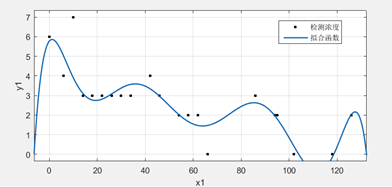
\includegraphics[width=\textwidth]{figures/1.png}

\end{figure}  

	\begin{figure}[H]
	\centering
	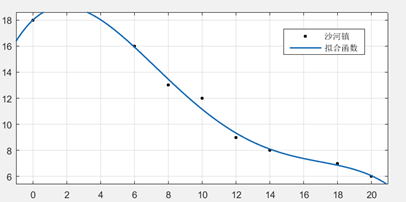
\includegraphics[width=\textwidth]{figures/2.png}

\end{figure} 

\end{document}